\documentclass[a4paper,12pt,oneside,openright,onecolumn,final,titlepage,fleqn,ngerman]{scrreprt}

% Gliederungsebenen:
% \part{}
% \chapter{}
% \section{}
% \subsection{}
% \subsubsection{}
% \paragraph{}
% \subparagraph{}

% Package definitions
\usepackage[ngerman]{babel}
\usepackage[utf8]{inputenc}

% package to control enumerations
\usepackage{enumerate}

% package to make the shorting table
\usepackage{longtable}
\renewcommand{\arraystretch}{1.5}

% use graphix
\usepackage{graphicx}

% for mathematical formula
\usepackage{amsmath}

% flushleft for caption
\usepackage{caption}

% use colors
\usepackage{color}
\definecolor{orange}{rgb}{1,0.784,0}
\definecolor{gray}{rgb}{0.5,0.5,0.5}

% package for killing borders at title page
\usepackage{geometry}

% Quotations
% \usepackage[numbers]{natbib}
\usepackage{multibib}
% \bibliographystyle{alphadin}

% other useful packages
\usepackage{tabularx}

% syntax highlighting
\usepackage{scrhack}		% makes a warning disappearing, but does dirty things!
\usepackage[final]{listings}
\lstset{
	frame=single,
	language=Java
}
\renewcommand{\lstlistingname}{Quelltext}
\renewcommand{\lstlistlistingname}{Quelltextverzeichnis}

% for links, LOAD AT LAST!
\usepackage[colorlinks,
pdfpagelabels,
pdfstartview = FitH,
bookmarksopen = true,
bookmarksnumbered = true,
linkcolor = black,
plainpages = false,
hypertexnames = false,
citecolor = black] {hyperref}

% set bibliographies
\newcommand{\refver}{Literaturverzeichnis}
\newcommand{\webver}{Verzeichnis der Webadressen}
\newcites{Refs,Urls}{\refver, \webver}

% disable indents for new paragraphs
\setlength{\parindent}{0cm}

% set header/footer
\usepackage{scrpage2}
\pagestyle{scrheadings}
% \setkomafont{pageheadfoot}{}		% set heading not italic
\automark{chapter}

\usepackage{tocloft}
\renewcommand{\cftfigpresnum}{Abb. }
\renewcommand{\cftfigaftersnum}{:}
\settowidth{\cftfignumwidth}{Abb. 8.88\quad}

% set new symbol for itemize-environment
\renewcommand{\labelitemi}{--}

% set depth of toc (depth=3, starts at 0!)
\setcounter{tocdepth}{2}

% important commands
\newcommand{\parag}{\\[2ex]}
\newcommand{\zB}{z.\,B.}
\newcommand{\abkEntry}[2]{\textbf{#1} & #2\\}
\newcommand{\imgCaption}[2]{\caption[#1]{#1 (\textit{Quelle:} #2)}}			% to define the sources of images

% set some constants
\newcommand{\calcag}{Berechnungsagent}
\newcommand{\coordag}{Koordinationsagent}
\newcommand{\repag}{Darstellungsagent}
\newcommand{\numag}{Numerikagent}
\newcommand{\iteag}{ITE-Agent}

\renewcommand{\ttdefault}{pcr}

% Document
\begin{document}
\bibliographystyleRefs{plaindin}
\bibliographystyleUrls{urls}
	% setting roman counter for toc,...
	\pagenumbering{Roman}

	% title page
	\begin{titlepage}
		% kill borders for title page
		\newgeometry{
			left=1cm,
			right=1cm,
			top=2cm,
			bottom=1cm,
			bindingoffset=5mm
		}

		\begin{center}
			\begin{tabularx}{\textwidth}{rXcXl}
				\begin{tabular}{c}
\includegraphics[keepaspectratio=true,height=0.15\textwidth]{res/unilogo.png} \end{tabular} & &
				\large\begin{tabular}{c}
					Universität Stuttgart\\
					Institut für Theorie der Elektrotechnik\\
					Prof. Dr. techn. Wolfgang M. Rucker
				\end{tabular}
				& & \begin{tabular}{c} 
\includegraphics[keepaspectratio=true,height=0.15\textwidth]{res/itelogo.png} \end{tabular}
			\end{tabularx}
	
			\vspace{20ex}

			{\Large\scshape Bachelorarbeit}
	
			\vspace{15ex}
	
			{\huge\bfseries Entwicklung eines Softwareagenten zur Darstellung der Prozessparameter numerischer Simulationen}
	
			\vspace{6ex}
	
			{\huge Development of an Software Agent for Presenting Numerical Simulation Process Parameters}
	
			\vspace{20ex}
	
			{\Large Fabian Diener}
	
			\vspace{23ex}
	
			\begin{tabbing}
				Abgabe der Ausarbeitung: \quad \= Dipl.-Ing. Matthias Jüttner\kill\\
				Betreuer: \> Dipl.-Ing. Matthias Jüttner\\[0.5ex]
				Beginn der Arbeit: \> 01.04.2014\\[0.5ex]
				Abgabe der Ausarbeitung: \> 13.11.2014
			\end{tabbing}
		\end{center}
	\end{titlepage}

	% restore borders for rest of document
	\restoregeometry
	\newgeometry{bindingoffset=5mm}		% set offset for binding the whole  later

	% begin with text on the next odd page
	\thispagestyle{empty}
	\cleardoublepage

	% preface
	\chapter*{Erklärung}
	\addcontentsline{toc}{chapter}{Erklärung}
	Hiermit erkläre ich,

	\begin{itemize}
		\item dass ich die vorliegende Arbeit selbstständig verfasst habe,
		\item dass ich keine anderen als die angegebenen Quellen und alle wörtlich oder sinngemäß aus anderen Werken übernommenen Aussagen als solche gekennzeichnet habe,
		\item dass die eingereichte Arbeit weder vollständig noch in wesentlichen Teilen Gegenstand eines anderen Prüfungsverfahrens ist,
		\item dass ich die Arbeit noch nicht veröffentlicht habe,
		\item dass das elektronische Exemplar mit diesem Exemplar übereinstimmt.
	\end{itemize}

	\bigskip

	Stuttgart, den 13.11.2014

	\newpage
	
	\chapter*{Abkürzungsverzeichnis}
	\addcontentsline{toc}{chapter}{Abkürzungsverzeichnis} % entry to toc
	\begin{longtable}{rl}
		\abkEntry{ACL}{Agent Communication Language (siehe \citeRefs{jade})}
		\abkEntry{CA}{\calcag{} (CalculationAgent)}
		\abkEntry{CPU}{Central Processing Unit}
		\abkEntry{FIPA}{Foundation for Intelligent Physical Agents}
		\abkEntry{GPL}{General Public License}
		\abkEntry{GUI}{Graphical User Interface -- Benutzeroberfläche}
		\abkEntry{ID}{IDentifikator}
		\abkEntry{ITE}{Institut für Theorie der Elektrotechnik}
		\abkEntry{JADE}{Java Agent DEvelopment framework}
		\abkEntry{LGPL}{Lesser General Public License}
		\abkEntry{PC}{Personal Computer}
		\abkEntry{PDF}{Portable Document Format}
		\abkEntry{RA}{\repag{} (ReportAgent)}
		\abkEntry{RAM}{Random Access Memory -- Arbeitsspeicher}
		\abkEntry{SIGAR}{System Information Gatherer And Reporter}
		\abkEntry{SMS}{Short Message Service}
	\end{longtable}

	\chapter*{\abstractname}
	\addcontentsline{toc}{chapter}{\abstractname}
	In der folgenden Arbeit wird ein Programm zur Erfassung und Darstellung von Prozessparametern einer Rechner-Plattform zur Lösung numerischer Simulationen vorgestellt. Dieses soll möglichst einfach in der Bedienung sein, einen guten Überblick über die gesamte Plattform bieten und die erfassten Prozessparameter in geeigneter Weise darstellen.\parag{}
	Im Folgenden wird ein möglicher Lösungsansatz für diese Anforderungen beschrieben. Da das hier entwickelte Programm die Schnittstelle zwischen Benutzer und Rechner darstellt, wird auf eine gute Bedienbarkeit der Benutzeroberfläche besonderen Wert gelegt. Es gelingt, die Prozessparameter intuitiv interpretierbar zu präsentieren. Die Entwicklung des Programms geschieht nach dem Wasserfallmodell\footnote{lineares Vorgehensmodell in der Softwaretechnik (siehe \citeRefs{info2})}.

	% table of contents
	\clearpage		% flush page before printing toc -> toc to new page
	\tableofcontents
% 	\addcontentsline{toc}{chapter}{\contentsname}		% add toc to toc ;)
	
	% set new page numbering
	\pagenumbering{arabic}
	
	\chapter{Einleitung}
	Die Entwicklung technischer Geräte aller Art, beispielsweise Autos oder Mobiltelefone, geschieht heute mithilfe von Simulationen. Da zur Perfektionierung dieser Geräte möglichst präzise Informationen benötigt werden, steigt die Komplexität der dazugehörigen Simulationsmodelle. Hierdurch steigt auch der Rechenaufwand. Heutige Rechenleistung wird durch die Vernetzung einzelner Rechner zu sogenannten \emph{Clustern}\footnote{siehe \citeRefs{cluster}} generiert. Hierbei löst ein einzelner Rechner ein Teilproblem eines komplexen Gesamtsystems. Um in diesem Cluster die Kontrolle zu behalten, sind dedizierte Programme erforderlich. Ein solches Programm zur Überwachung und Kontrolle eines Rechner-Clusters in Form einer Agenten-Plattform für numerische Simulationen wird in dieser Arbeit vorgestellt. Zunächst werden die wesentlichen technischen Grundlagen erläutert, die für das Verständnis dieser Arbeit erforderlich sind. Da dies nur ein grober Über\-blick sein kann, wird für ein tieferes Verständnis eine präzisere Einarbeitung anhand der verwiesenen Referenzen empfohlen.
	
	\section{Software-Agenten}
	Bei einem (Software-)Agent handelt es sich um ein autonomes Programm, welches für eine bestimmte Aufgabe, die an die Software gestellt wird, benötigt wird. Der Zusammenhalt der einzelnen Agenten zur bedienbaren Software geschieht hierbei durch ein Nachrichtensystem (siehe dazu Kapitel \ref{kap_messageSystem}). Hierdurch wird eine größere \emph{Kapselung}\footnote{Abschottung von Softwareteilen in der objektorientierten Programmierung} der einzelnen Teilbereiche der Software geschaffen, als es durch objektorientierte Programmierung möglich wäre. Dies erhöht wiederum das Abstraktionsniveau und wird daher auch als die logische Fortsetzung der bisherigen Programmierentwicklung gesehen\footnote{siehe \citeRefs{info2}}.
	
	\section{Java}
	Java ist eine objektorientierte Programmiersprache. Sie wird für die Realisierung des Programms benötigt. Eine gute Einführung ist in \citeRefs{java} zu finden.
	
	\section{JADE}\label{kap_jade}
	Das Java Agent DEvelopment framework\footnote{siehe \citeRefs{jade}} (JADE) implementiert ein Agentensystem, welches die Spezifikationen der Foundation for Intelligent Physical Agents (FIPA) als Java-Plattform zur Verfügung stellt. Durch die Einhaltung des Standards wird dabei eine Kompatibilität mit anderen Agenten gewährleistet, welche nicht unbedingt in Java implementiert sein müssen. Mit JADE können einzelne Agenten beliebig angehalten und fortgesetzt werden, sogar die Portierung auf andere Rechner zur Laufzeit wird gestattet. Letzteres erlaubt eine bessere Ressourcennutzung durch eine bessere Verteilbarkeit des Rechenaufwandes.

	\section{Struktur der existierenden Plattform}\label{kap_existingPlatform}
	Das ITE betreibt eine Agenten-Plattform zur Berechnung elektrotechnischer Probleme. Der Agent zur Darstellung der Prozessparameter numerischer Simulationen ist in diese, bereits bestehende Plattform eingebettet. Diese ist, wie in Abbildung \ref{overview} dargestellt, aufgebaut.
	\begin{figure}[ht]
		\centering
		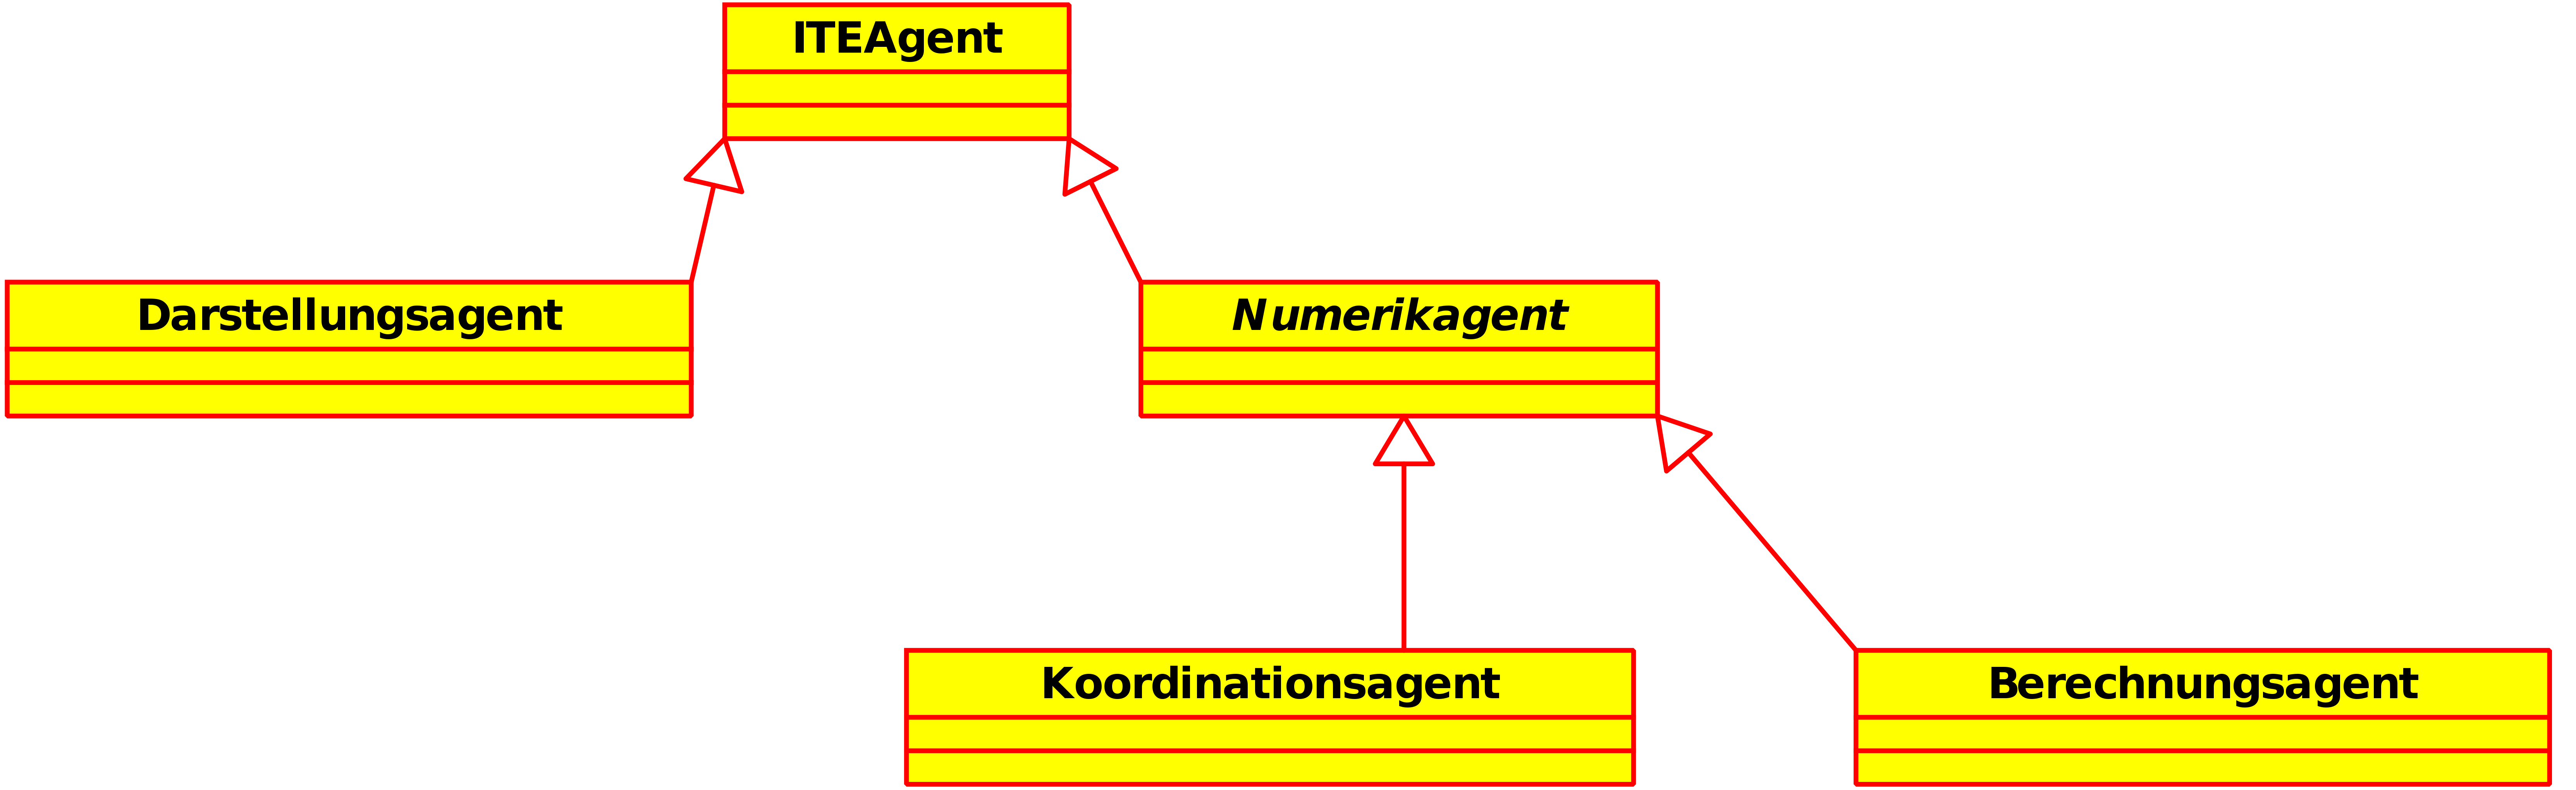
\includegraphics[keepaspectratio=true,width=\textwidth]{res/overview.png}
		\caption[Überblick über das bisherige Agenten-System]{Überblick über das bisherige Agenten-System, \emph{nach Vorlage von Dipl.-Ing. Matthias Jüttner}}
		\label{overview}
	\end{figure}
	
	Der \iteag{} ist die Basis aller weiteren Agenten. Der \numag{}, der den Berechnungszweig beginnt und sich klar von dem \repag{}en abgrenzt, erbt vom \iteag{} und ist wiederum Grundlage für \calcag{} und \coordag{}. Der \repag{} erbt ebenfalls vom \iteag{} und übernimmt die Darstellung der Prozessparameter. Der \calcag{} löst ein Teilproblem des Modells, während der \coordag{} die verschiedenen \calcag{}en koordiniert. Es ist im Allgemeinen davon auszugehen, dass eine Instanz\footnote{Im Allgemeinen ein Objekt, durch den agentenorientierten Ansatz jedoch eher als Teilprogramm zu verstehen} des \coordag{}en und \repag{}en, jedoch mehrere Instanzen des \calcag{}en existieren. Alle Agenten nutzen zur Darstellung denselben \repag{}en.\parag{}
	Da der \repag{} allgemein eingesetzt werden kann, sei an dieser Stelle erwähnt, dass dieser vom \iteag{} im Wesentlichen die Funktion erbt, andere Agenten in der Agentenplattform zu suchen. Soll der \repag{} auf eine andere Plattform übertragen werden, so muss ihm diese Fähigkeit verliehen werden.
	
	\subsection{Nachrichtensystem}\label{kap_messageSystem}
	Die Kommunikation unter den Agenten geschieht über Nachrichten, sogenannte \emph{ACLMessages} (Agent Communication Language Messages). Dieses in \mbox{JADE} implementierte Nachrichtensystem transportiert Textnachrichten in Form von  \emph{Strings} oder ganze Objekte\footnote{Der Transport von Objekten ist nicht FIPA-konform und sollte daher vermieden werden. \citeRefs{jade}}. Dabei trägt jede Nachricht eine \emph{Conversation-ID}. Diese ist als \emph{String} realisiert. Sie wird in der Kommunikation mit dem \repag{}en durch das Protokoll (siehe Kapitel \ref{kap_protocol}) definiert und verwendet, um dem \repag{}en die Bedeutung der Nachricht mitzuteilen, \zB{} ob ein neuer Prozessparameter registriert werden soll.

	\chapter{Prozessparameter}\label{kap_parameter}
	Prozessparameter, die in numerischen Simulationen zur Auswertung zur Ver\-fü\-gung stehen, existieren reichlich. Um die Übersichtlichkeit zu gewährleisten, ist eine Beschränkung auf die \emph{wesentlichen} Prozessparameter ratsam. Dabei hängt der Begriff \glq{}wesentlich\grq{} jedoch vom jeweiligen Umfeld ab.
	
	Die Prozessparameter, die hier an dieser Stelle erfasst werden, lauten:
	\begin{itemize}
		\item \textbf{Fortschritt}\\Der Berechnungsfortschritt des jeweiligen Teilproblems
		\item \textbf{PC-Status-Monitor}\\Auslastung von Prozessor (CPU) und Arbeitsspeicher (RAM) des jeweiligen Rechners, der den \calcag{}en trägt
		\item \textbf{Mesh\footnote{Polygonnetz zur Diskretisierung mehrdimensionaler Modelle}-Daten}\\Informationen über die Meshes des Modells
		\item \textbf{Konvergenzdaten}\\Daten, die den Iterationsfehler in Abhängigkeit des Interationsschritts be\-in\-hal\-ten. Diese Daten sind damit ein Maß für die Konvergenz des iterativen Lösungsverfahrens.
	\end{itemize}
	
	\chapter{Analyse}\label{kap_analyse}
	Der Agenten zur Darstellung von Prozessparameter numerischer Simulationen ist ein Agent, der ausschließlich für die Interaktion mit dem Benutzer vorgesehen ist. Daher hat er vor allem nachfolgende Aufgaben zu bewältigen
	
	\begin{enumerate}[\protect{A}1: ]
		\item Einfache, möglichst  \emph{intuitive Bedienbarkeit}
		\item Darstellung der Prozessparameter in adäquater Weise. Diese hat nach Mög\-lich\-keit aufgrund der einfacheren Erfassbarkeit in Form von Diagrammen zu erfolgen.
		\item \emph{Robustheit} gegenüber Programmierfehlern. Ein Abstürzen, Einfrieren oder sonstiges von der Norm abweichendes Verhalten ist für den \repag{}en nicht tolerierbar.
	\end{enumerate}
	
	Der Agent beschränkt sich also auf die Darstellung der Prozessparameter. Eine Auswertung dieser in Kombination mit einem autonomen Verhalten stellen interessante Erweiterungsmöglichkeiten dar und werden in Kapitel \ref{kap_ausblick} näher beleuchtet.
	
	\section{Benutzeroberfläche}\label{kap_ana_gui}
	Bei der Entwicklung der Benutzeroberfläche (GUI) wird nach oben erwähnten Anforderungen vor allem auf folgende Punkte Wert gelegt:
	\begin{itemize}
		\item \emph{Übersichtlichkeit}
		\item \emph{Einfache Bedienbarkeit}
		\item \emph{Einfache Vergleichbarkeit} der Daten
		\item \emph{Dynamik}: Die GUI muss in der Lage sein, neue Daten zur Laufzeit und während des Berechnungsprozesses anzuzeigen bzw. zu aktualisieren. Ist sie dies nicht, so erweckt sie schnell den Eindruck, die gesamte Agentenplattform wäre untätig.
	\end{itemize}
	
	\chapter{Entwurf des Agenten}\label{kap_entwurf}
	In diesem Kapitel wird der Entwurf des Agenten vorgestellt. Kapitel \ref{kap_implementation} beschreibt die Implementierung des Agenten und setzt die in diesem Kapitel gewonnenen Erkenntnisse um.
	
	\section{Einsatz von Komponenten}
	Beim Entwurf des Agenten, spätestens jedoch bei dessen Implementierung, muss entschieden, ob Software-Komponenten eingesetzt werden oder nicht. An dieser Stelle fällt die Entscheidung für die Software-Komponenten, da diese die Software-Qualität verbessern und den Implementierungsaufwand verringern\footnote{siehe \citeRefs{info2}, \citeRefs{swQuali}}.
	
	\section{Benutzeroberfläche}
	Der Entwurf der GUI wird in diesem Kapitel vorgestellt. Die Anforderungen hierzu sind in Kapitel \ref{kap_ana_gui} aufgeführt. Diese legen hierbei eine hierarchische Struktur nach Abbildung \ref{img_strukt_gui} nahe.
	\begin{figure}[ht]
		\centering
		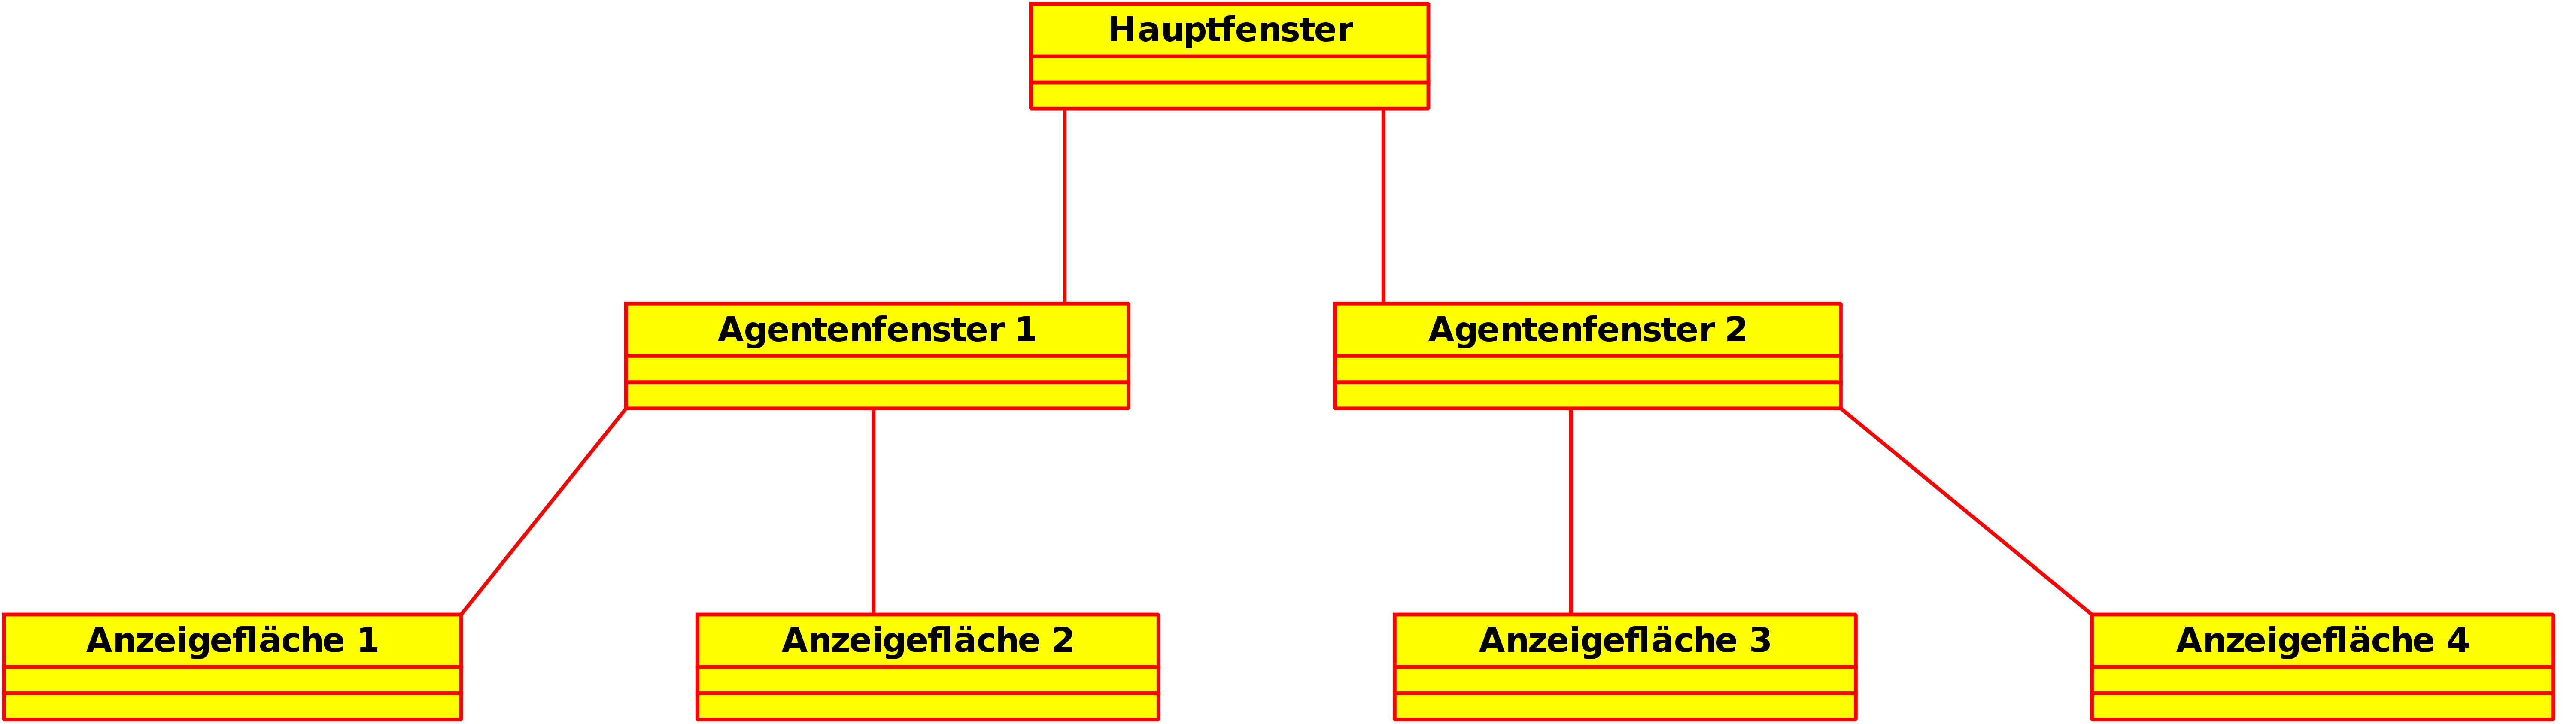
\includegraphics[keepaspectratio=true,width=\textwidth]{res/Struktur_GUI.png}
		\caption{Hierarchische Struktur der Benutzeroberfläche}
		\label{img_strukt_gui}
	\end{figure}
	
	Die \emph{Vergleichbarkeit} fordert, dass mehrere Graphen über-, in- oder zumindest nebeneinander dargestellt werden können. Die \emph{Übersichtlichkeit} wird insofern berücksichtigt, als jedem Agenten ein eigenes Teilfenster zugewiesen wird. Dieser Ansatz trennt die einzelnen Agenten klar voneinander ab und lässt sofort Rückschlüsse zu, welcher Prozessparameter zu welchem Agenten gehört. Durch separierte Fenster wird auch die \emph{Vergleichbarkeit} von Prozessparameter zwischen verschiedenen Agenten gewährleistet. Die \emph{Bedienbarkeit} und \emph{Dynamik} werden hier nicht durch einen bestimmten Ansatz verfolgt, werden jedoch bei der Implementierung in Kapitel \ref{kap_implementation} beachtet. Die Zuweisung der jeweiligen Diagramme zu den Agentenfenstern ist dabei notwendig und wird in einfacher Form vorgenommen.
	
	\section{Datenerhebung}
	Die Datenerhebung, also das Ermitteln der Prozessparameter, geschieht nicht im \repag{} selbst, sondern erfolgt außerhalb -- in der in Kapitel \ref{kap_existingPlatform} vorgestellten Plattform im \calcag{}. Sie ist der Vollständigkeit halber dennoch erwähnt, wobei eine Beschränkung auf die Implementierungsdetails (Kapitel \ref{kap_implementation}) stattfindet.
	
	\section{Prozessparameter-Verwaltung}\label{kap_entw_parver}
	Verwaltet werden die Prozessparameter, die in Kapitel \ref{kap_parameter} erwähnt sind. Dabei geschieht die Verwaltung eines Prozessparameters prinzipiell wie in Abbildung \ref{seq_parver} dargestellt.
	\begin{figure}[ht]
		\centering
		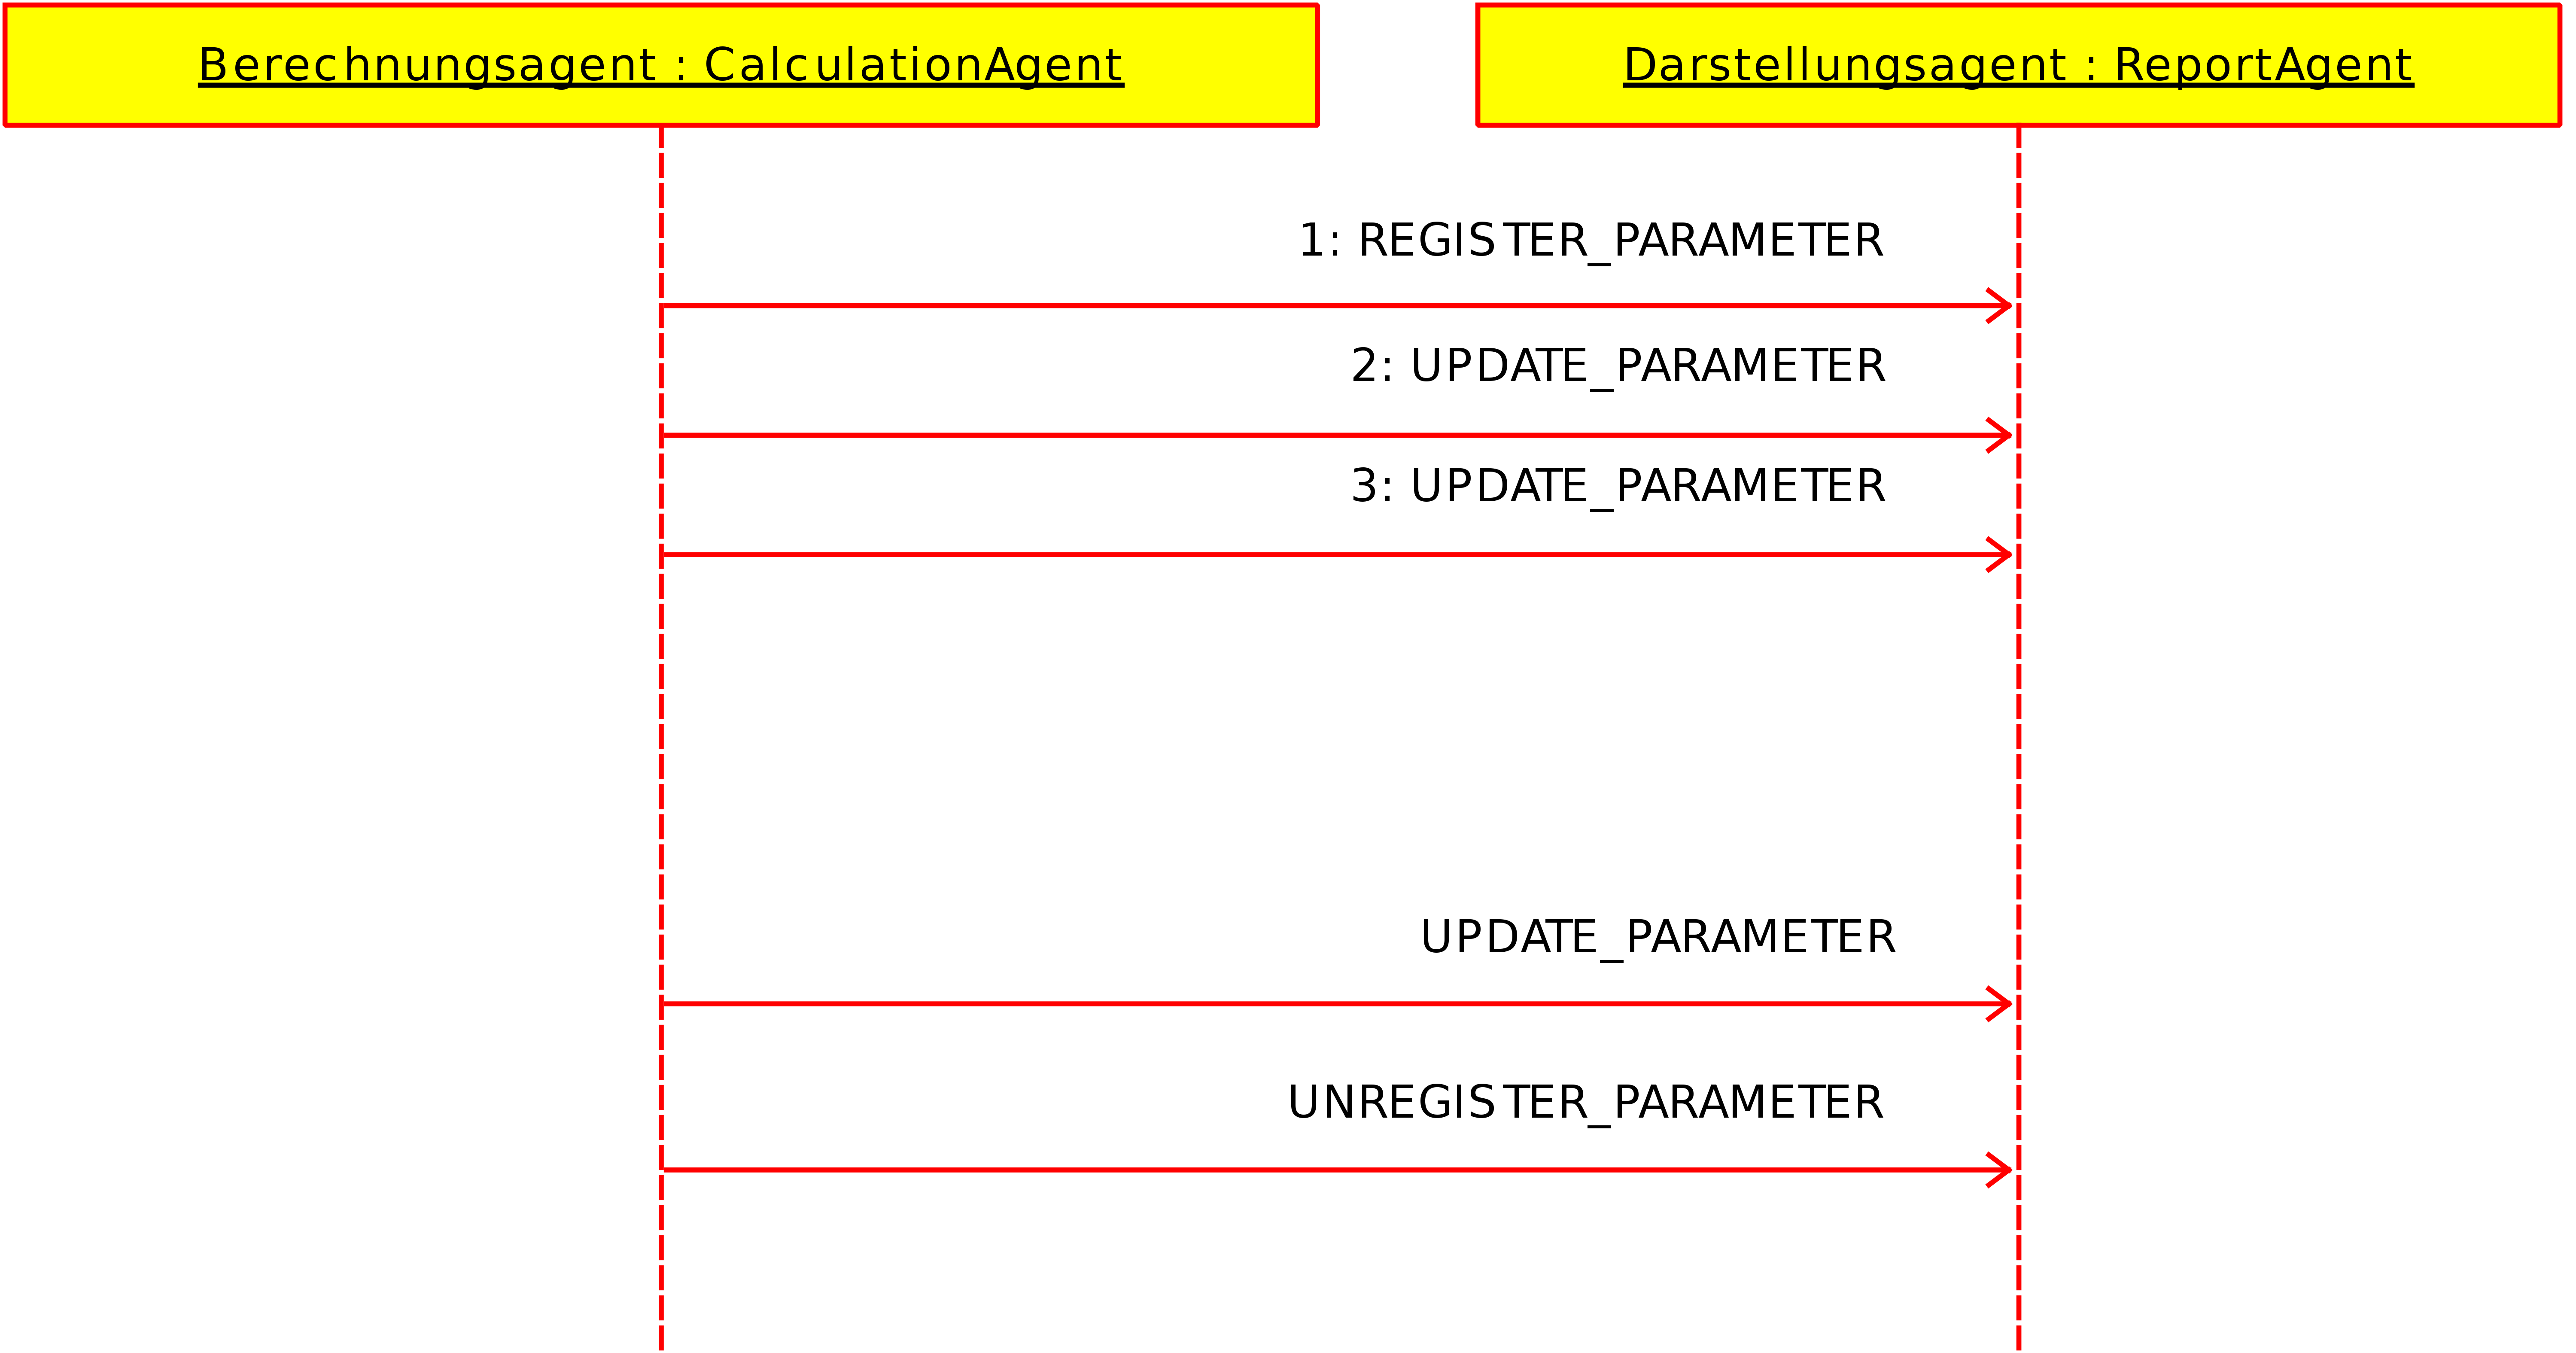
\includegraphics[keepaspectratio=true,width=\textwidth]{res/Sequenzdiagramm_Parameterverwaltung.png}
		\caption{Prinzipielle Prozessparameterverwaltung}
		\label{seq_parver}
	\end{figure}
	Zunächst wird ein Prozessparameter beim \repag{}en \emph{registriert}. Anschließend besteht die Möglichkeit durch \emph{Updates} einem bestehenden Prozessparameter Daten hinzuzufügen. Wird der Prozessparameter nicht mehr benötigt, so kann er durch \emph{Deregistrierung} wieder entfernt werden. Durch diesen Entwurfsansatz ist die einfache Erweiterbarkeit durch neue Prozessparameter gegeben. Es ist zu betonen, dass jeder Agent lediglich in der Lage ist, die Prozessparameter zu manipulieren, die er selbst registriert hat. Dies fördert die \emph{Robustheit} des Programms, da sich eventuelle Fehler eines \calcag{}en nicht auf den gesamten \repag{}en ausdehnen können und dürfen.
	
	\chapter{Implementierung des Agenten}\label{kap_implementation}
	Im Folgenden wird die Entwicklung des \repag{}en beschrieben. Dabei werden die Erkenntnisse aus Kapitel \ref{kap_entwurf} umgesetzt. Die hier vorgestellte Implementierung ist dabei nur eine Möglichkeit von vielen.

	\section{Eingesetzte Komponenten}
	Im Entwurf in Kapitel \ref{kap_entwurf} wurde die Entscheidung für den Einsatz von Komponenten gefällt. Im Folgenden werden die eingesetzten Komponenten vorgestellt.
	
	\subsection{DockingFrames}\label{kap_DockingFrames}
	\begin{figure}[ht]
		\centering
		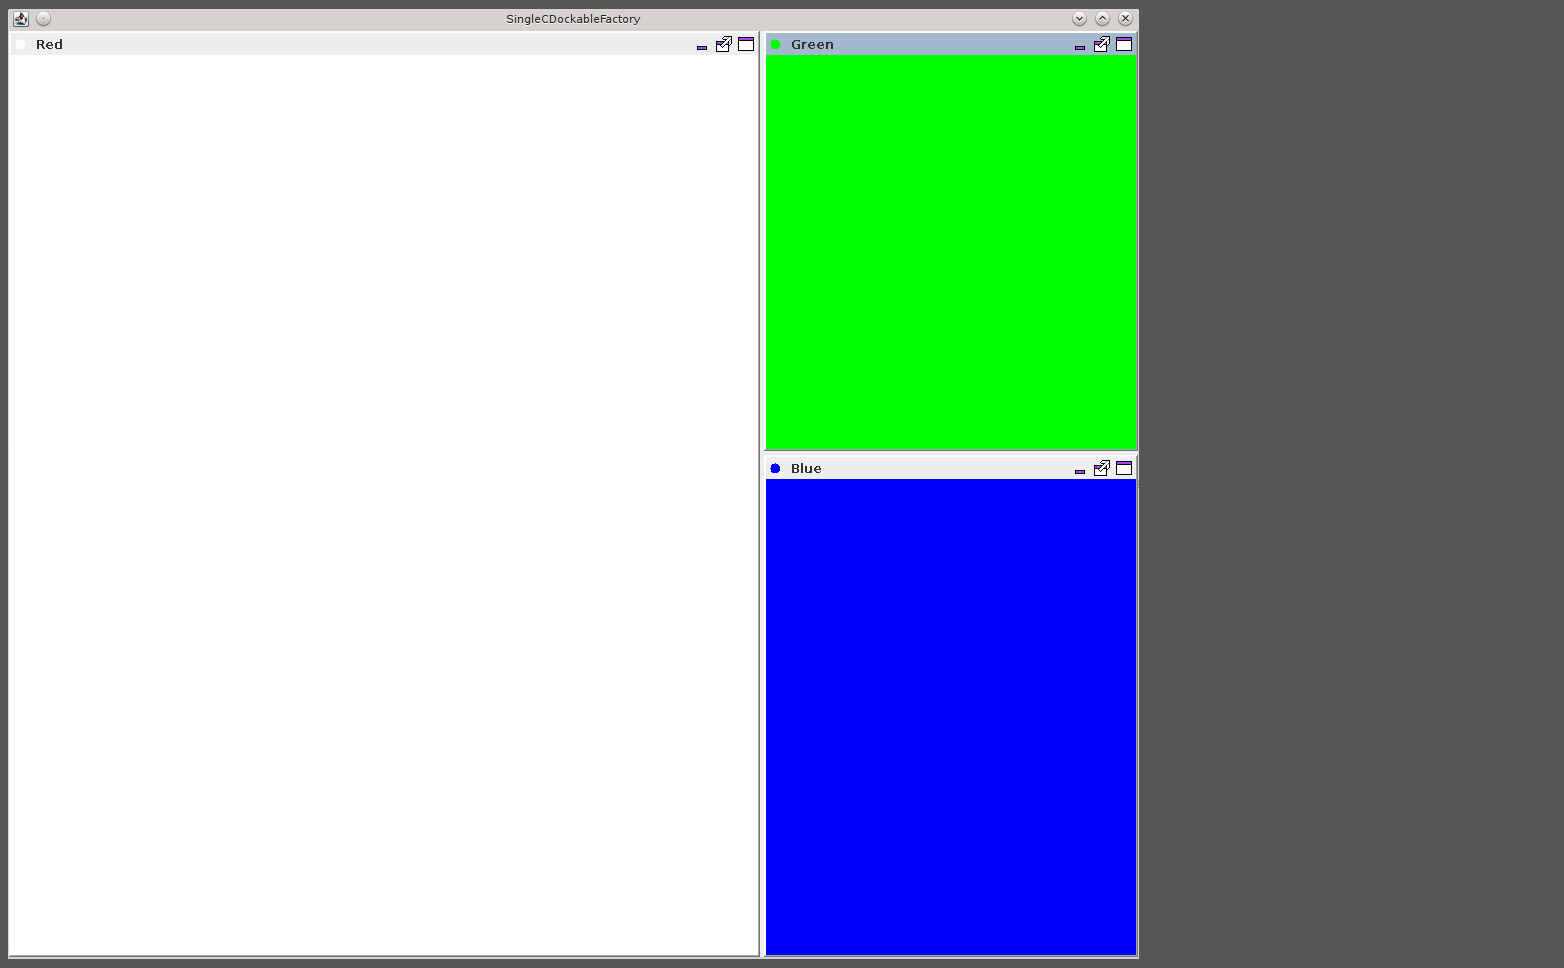
\includegraphics[keepaspectratio=true,width=0.8\textwidth]{res/DF_int.png}
		\caption{DockingFrames-Beispiel}
		\label{pic_df_int}
	\end{figure}
	
	\begin{figure}[ht]
		\centering
		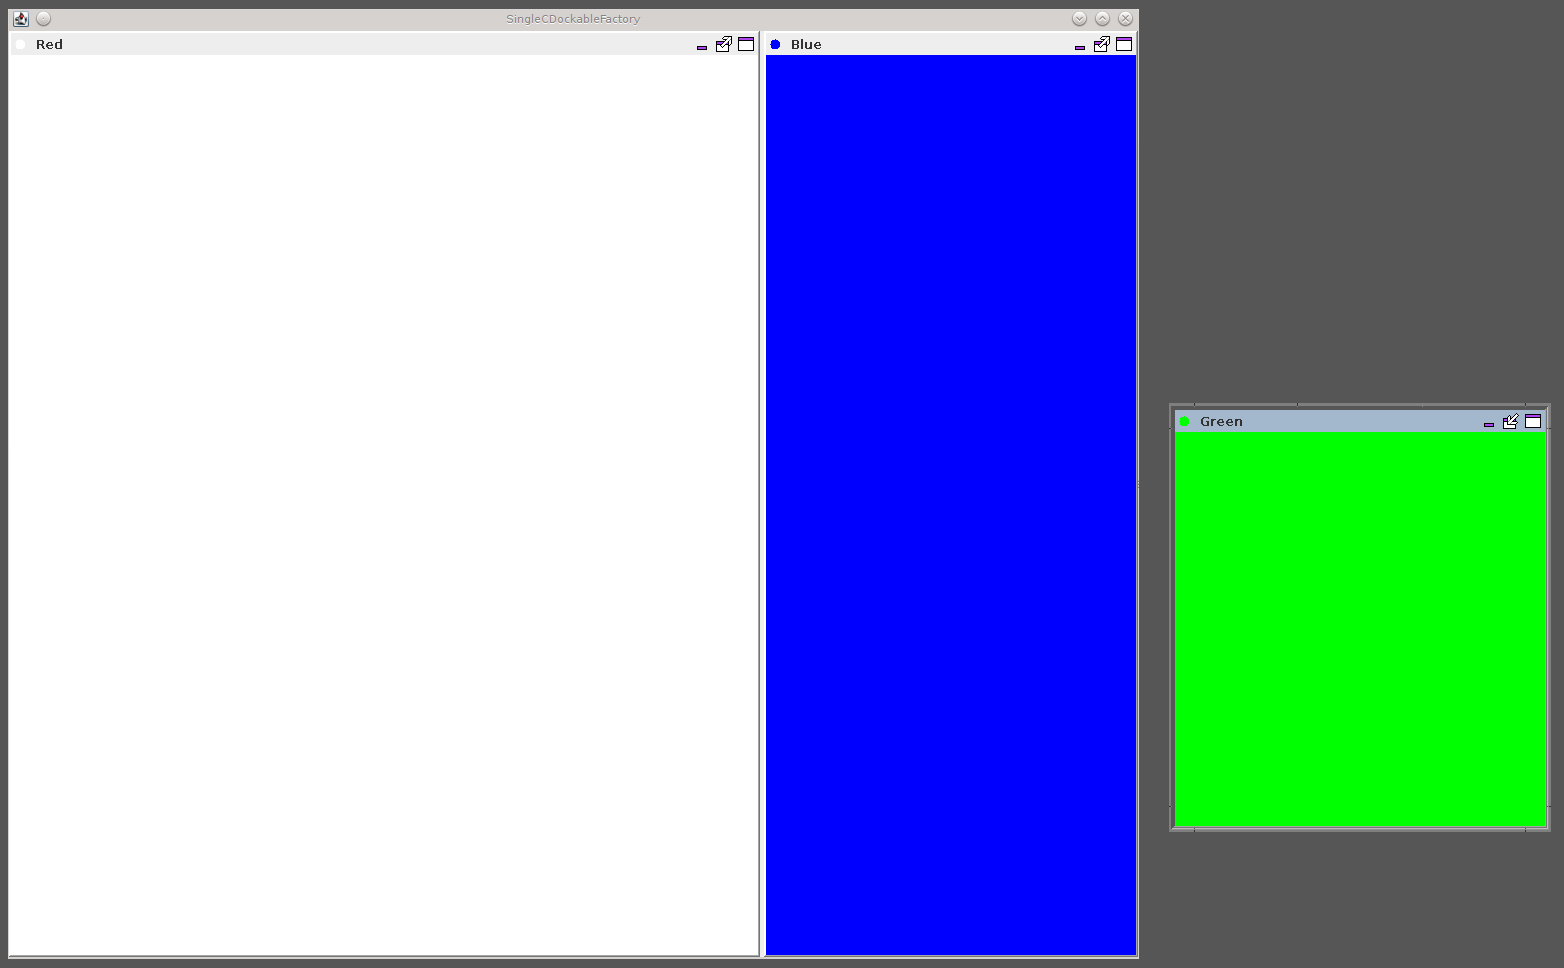
\includegraphics[keepaspectratio=true,width=0.8\textwidth]{res/DF_ext.png}
		\caption{DockingFrames-Beispiel mit ausgedocktem Fenster}
		\label{pic_df_ext}
	\end{figure}
	DockingFrames\footnote{Projektseite: \citeUrls{DF}} stellt Fenster als sogenannte \emph{Dockables} dar. Ein Dockable ist dabei ein Unterfenster, welches eine beliebige Positionierung auf dem Bildschirm gestattet. Es ist vom Hauptfenster lösbar und lässt sich jederzeit wieder in dieses integrieren, wie in Abbildung \ref{pic_df_int} und \ref{pic_df_ext} dargestellt. Dieses Projekt erfüllt damit viele Anforderungen, die im Entwurf der GUI gefordert wurden. Das Projekt ist unter der  Lesser General Public License (LGPL) veröffentlicht.
	
	\subsection{JFreeChart}\label{kap_JFreeChart}
	\begin{figure}[ht]
		\centering
		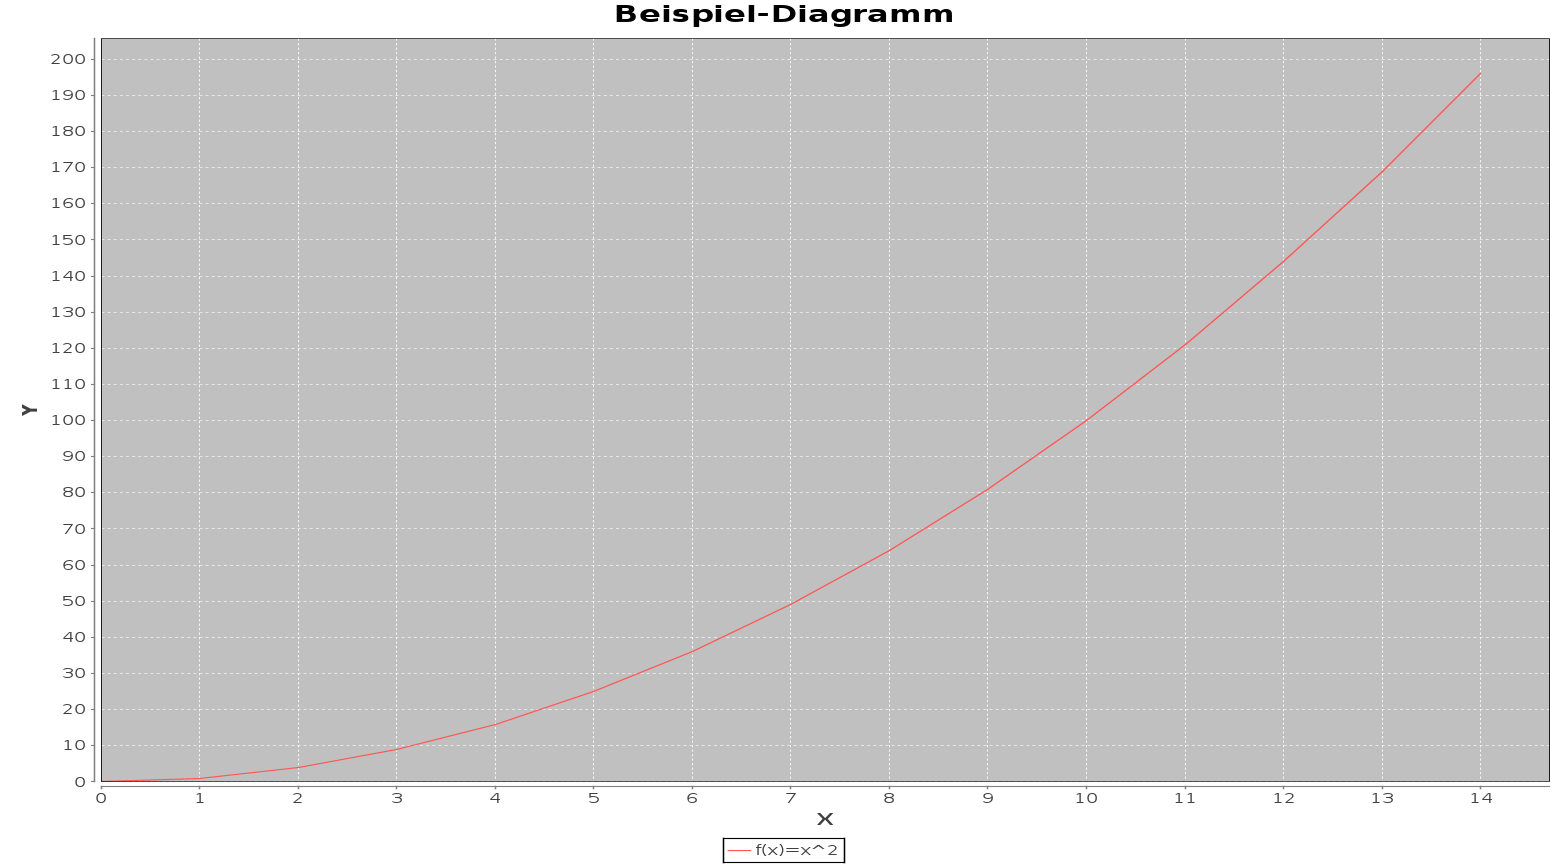
\includegraphics[keepaspectratio=true,width=0.8\textwidth]{res/jfc_bsp.png}
		\caption{Beispiel-Diagramm, mit JFreeChart gezeichnet}
		\label{pic_jfc_bsp}
	\end{figure}
	JFreeChart\footnote{Projektseite: \citeUrls{JFC}} ist ein Projekt, mit dem Diagramme gezeichnet werden können. Es werden die verschiedensten Diagrammtypen unterstützt, beispielsweise Balkendiagramme, Kreisdiagramme oder -- von dem \repag{}en häufig benötigt -- XY-Diagramme. Ein Beispiel-Diagramm ist in Abbildung \ref{pic_jfc_bsp} abgebildet. JFree\-Chart ist ebenfalls unter der LGPL veröffentlicht.
	
	\subsection{SIGAR}\label{kap_sigar}
	Der System Information Gatherer And Reporter (SIGAR)\footnote{Projektseite: \citeUrls{SIG}} stellt eine betriebssystemunabhängige Schnittstelle für Systemressourcen-Informationen unter Java zur Verfügung. Dieses Paket wird dazu verwendet, CPU- und RAM-Auslastung anzuzeigen und findet bei dem später vorgestellten PC-Status-Monitor Verwendung. Das Projekt ist unter der Apache-Lizenz Version 2 veröffentlicht.
	
	\section{Benutzeroberfläche}\label{kap_impl_gui}
	Im Folgenden wird die Umsetzung der Erkenntnisse für die GUI aus Kapitel \ref{kap_entwurf} vorgestellt.
	
	\subsection{Hauptfenster}
	\begin{figure}[ht]
		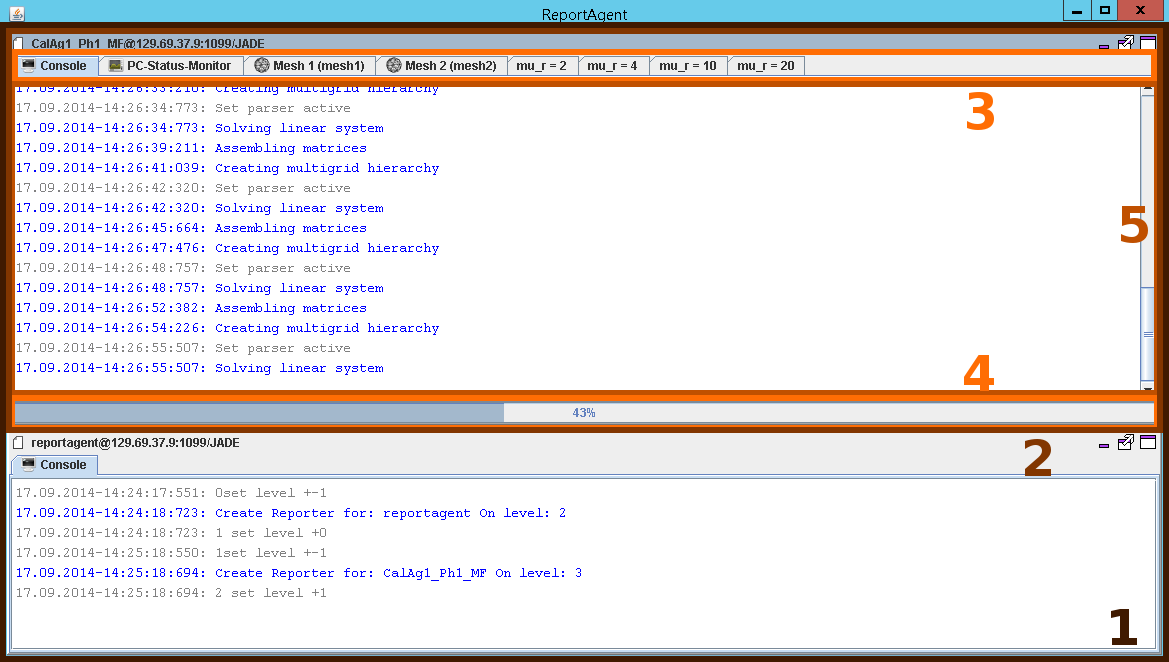
\includegraphics[keepaspectratio=true,width=\textwidth]{res/MainWin.png}
		\caption{GUI des  \repag{}en (Hauptfenster)}
		\label{repag_mainwin}
	\end{figure}
	Das Hauptfenster ist durch die Swing-Klasse \emph{JFrame} realisiert und in Abbildung \ref{repag_mainwin} abgebildet. Dieses bildet die Basis der GUI des \repag{}en.\parag{}
	Das Hauptfenster (1) beinhaltet alle Komponenten, wobei einzelne Agentenfenster (2) auch in der Lage sind, dieses zu verlassen. Pro Agent existiert ein Agentenfenster mit mehreren Tabs (3). Diese Tabs listen einzelne Prozessparameter eines Agenten auf -- in Abbildung \ref{repag_mainwin} sind es beispielsweise der PC-Status-Monitor, zwei Meshes, sowie mehrere Konvergenzdiagramme. Der Fortschrittsbalken (4) ist nur dann dargestellt, wenn er benötigt wird; er wird ausgeblendet, sobald die Berechnung vollständig abgeschlossen ist. Die Anzeigefläche (5) stellt den momentan gewünschten Prozessparameter dar. Die Konsole ist nicht als Prozessparameter geführt und ist stets der erste Tab. Darauf wird in Kapitel \ref{kap_impl_konsole} eingegangen.
	
	\subsection{Agentenfenster}\label{kap_impl_agwin}
	Das Agentenfenster wird durch einen Fenster-Typ des DockingFrames-Pro\-jektes (siehe Kapitel \ref{kap_DockingFrames}) realisiert. Dieser Fenster-Typ heißt \emph{Dockable}, da sie die Fähigkeit besitzen, sich in das Hauptfenster \glqq{}ein- oder auszudocken\grqq{}, also die Fähigkeit, sich flexibel zu lösen und neu anzuordnen. Dies veranschaulicht Abbildung \ref{pic_df_int} und \ref{pic_df_ext} aus Kapitel \ref{kap_DockingFrames}. Hierdurch wird ein flexibler Vergleich von Prozessparametern verschiedener Agenten ermöglicht. Darüber hinaus sind die Agentenfenster in sich geschlossen, was die Wahrnehmung der Autonomie einzelner Agenten stärkt.\parag{}
	Das Agentenfenster ist aufgeteilt in eine Anzeigefläche, die durch Tabs verändert werden kann, sowie eine Fortschrittsanzeige am unteren Bildschirmrand. Diese Aufteilung hat den Vorteil, dass der aktuelle Fortschritt der Berechnung stets eingesehen werden kann.
	
	\subsection{Anzeigefläche}
	Das Agentenfenster beinhaltet eine oder mehrere Anzeigeflächen. Die einzelnen Anzeigeflächen werden in demselben Agentenfenster angezeigt. Das Umschalten erfolgt über Registerkarten, \emph{Tabs} genannt. Die einzelnen Tabs sind -- mit Ausnahme der Konsole -- durch einen Rechtsklick schließbar. Das gezielte Schließen einzelner, nicht benötigter Tabs erhöht die Übersichtlichkeit der GUI. Die Möglichkeit, dies ohne Menü durch einen einfachen Rechtsklick zu erledigen, erleichtert die Bedienbarkeit.

	\subsubsection{Konsole}\label{kap_impl_konsole}
	Der erste Tab beinhaltet die Konsole des jeweiligen Agenten. Dies ist auch durch ein entsprechendes Icon (siehe Abbildung \ref{icon_console}) dargestellt.
	\begin{figure}[ht]
		\centering
		
\includegraphics[width=64px]{res/console.png}
		\imgCaption{Konsole-Icon}{\citeUrls{IKo}}
		\label{icon_console}
	\end{figure}
	
	\paragraph{Bedeutung}
	Die Konsole nimmt eine herausragende Bedeutung ein. Sie ist unverzichtbar, da sie folgende Aufgaben erfüllt:
	\begin{itemize}
		\item Ausgabe der Informationen während der numerischen Lösung
		\item Anzeige von Status- und Fehlermeldungen
		\item Ausgabesystem im Fehlerfall der GUI
	\end{itemize}
	
	Da diese Aufgaben von hoher Bedeutung sind, ist es nicht möglich, die Konsole zu schließen. Zur besseren Übersichtlichkeit werden die einzelnen Meldungen ihrer \emph{Wichtigkeit} nach formatiert. Die \emph{Wichtigkeit} ist hierbei in den Text-Levels (siehe Anhang \ref{kap_textlevels}) eindeutig definiert. Die Formatierung sieht dabei aus wie Abbildung in \ref{fig_format} dargestellt.
	\begin{figure}[ht]
		\centering
		\ttfamily
		\textbf{\color{red}{Fatal}}\\
		\color{red}{Error}\\
		\textbf{\color{orange}{Warning}}\\
		\textbf{\color{blue}{Information important}}\\
		\color{blue}{Information casual}\\
		\color{gray}{Debug}\\
		\color{black}{Unknown}
		\caption{Formatierung der verschiedenen Text-Level}
		\label{fig_format}
	\end{figure}
	

	\subsubsection{Inhalt der weiteren Tabs}
	Die weiteren Tabs beinhalten Prozessparameter des Computers oder des numerischen Berechnungsprogramms. Diese werden im Folgenden vorgestellt.
	
	\paragraph{PC-Status-Monitor}\label{kap_PCStatusMonitor}
	Der \emph{PC-Status-Monitor} stellt die CPU- und Ar\-beits\-spei\-cher-Auslastung in einem Diagramm graphisch dar. Die Daten hierzu stellt das SIGAR-Projekt zur Verfügung (siehe Kapitel \ref{kap_impl_data_pcs}). Er benutzt zur Darstellung dieser Daten das Projekt \emph{JFreeChart} (siehe Kapitel \ref{kap_JFreeChart}) und ist durch das Icon aus Abbildung \ref{icon_statusmonitor} klar identifizierbar.
	\begin{figure}[ht]
		\centering
		
\includegraphics[width=64px]{res/sysmonitor.png}
		\imgCaption{Icon des PC-Status-Monitors}{\citeUrls{IMo}}
		\label{icon_statusmonitor}
	\end{figure}
	
	Ein Beispiel des Status-Monitors ist in Abbildung \ref{ss_statusmonitor} dargestellt. Hier erkennt man, dass die Berechnung nach ca. 135\,s beendet wurde.
	\begin{figure}[ht]
		\centering
		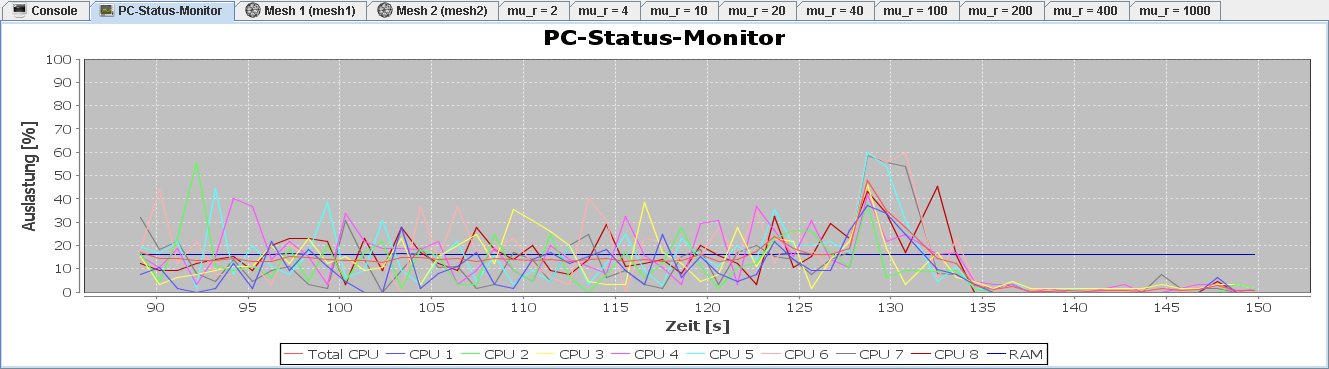
\includegraphics[keepaspectratio=true,width=\textwidth]{res/pcstatusmonitor.png}
		\caption{PC-Status-Monitor}
		\label{ss_statusmonitor}
	\end{figure}
	
	Es ist zu beachten, dass die Systemressourcen nicht einfach durch einen \emph{TaskManager} oder ein vergleichbares Tool überwacht werden können, da davon auszugehen ist, dass sich die Agenten auf verschiedenen Rechnern befinden. Der Status-Monitor stellt die Daten der Rechner, auf denen die \calcag{}en arbeiten, übersichtlich dar, wohingegen vergleichbare Tools lediglich den Rechner überwachen, auf dem sie selbst laufen.\parag{}
	Der Status-Monitor zeigt, wie bei vergleichbaren Tools üblich, die aktuellsten Messwerte an, hier in etwa die letzten 60 Sekunden. Überwacht wird in der ITE-Beispielplattform jeder Agent ausgenommen dem \repag{}en selbst. Dieser ist für diese Anwendung wenig interessant. Er ließe sich gegebenenfalls durch ein externes Tool überwachen, da der \repag{} stets auf dem Rechner, auf den der Benutzer zugreifen kann, läuft.

	\paragraph{Mesh-Daten}
	Da sich die Mesh-Daten nicht sinnvoll in einem Diagramm darstellen lassen, werden diese textuell ausgegeben. Dabei werden weitere nützliche Informationen wie Autor oder Bearbeitungsdatum angezeigt. Das Icon in der Tab-Leiste ist in Abbildung \ref{icon_mesh} dargestellt, ein Beispiel für eine Mesh-Ausgabe ist in Abbildung \ref{ss_mesh} zu sehen.
	\begin{figure}[ht]
		\centering
		
\includegraphics[width=64px]{res/mesh.png}
		\caption{Icon der Mesh-Statistik}
		\label{icon_mesh}
	\end{figure}
	\begin{figure}[ht]
		\centering
		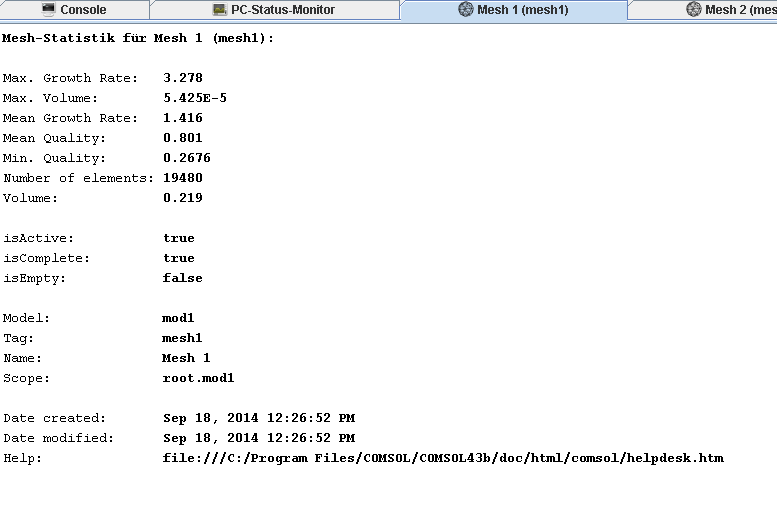
\includegraphics[keepaspectratio=true,width=\textwidth]{res/ss_mesh.png}
		\caption{Mesh-Statistik}
		\label{ss_mesh}
	\end{figure}
	
	\paragraph{Konvergenzdiagramme}
	Die Konvergenzdiagramme stellen den Iterationsfehler über die einzelnen Iterationsschritte dar (siehe Abbildung \ref{ss_konvplot}). Sie sind damit ein Indiz für den Fortschritt des Lösungsprozesses. Sie werden ebenfalls von \emph{JFreeChart} dargestellt, im Unterschied zum PC-Status-Monitor allerdings mit logarithmischer \(y\)-Achse.\parag{}
	Der Titel eines Konvergenzdiagrammes lautet \glqq{}\textless{}Solver-Typ\textgreater{} -- Konvergenzplot\grqq{}, wobei \emph{\textless{}Solver-Typ\textgreater{}} die Art des Lösungsverfahrens angibt, beispielsweise \glqq{}LinearSolver\grqq{}\footnote{Mehr dazu in Kapitel \ref{kap_impl_konvdata}}. Werden mehrere Parameter berechnet, so beschreibt der Titel den dargestellten Parameter -- wie in Abbildung \ref{ss_konvplot}. Hierbei sind die einzelnen Iterationsschritte diskret, zur besseren Übersichtlichkeit ist es jedoch üblich, die einzelnen Punkte durch lineare Interpolation zu einer Kurve zu verbinden.
	\begin{figure}[ht]
		\centering
		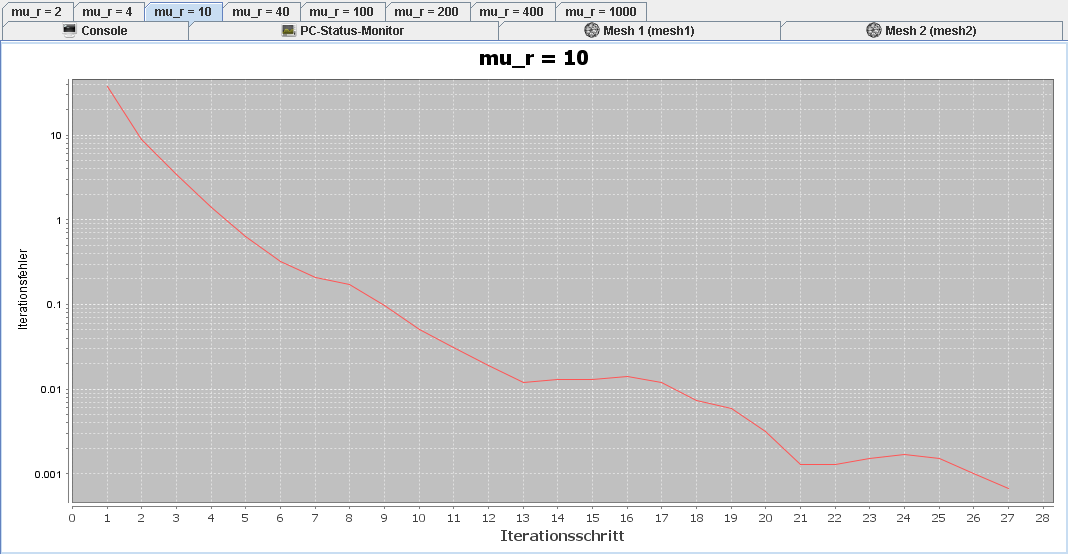
\includegraphics[keepaspectratio=true,width=\textwidth]{res/ss_konvplot.png}
		\caption{Beispiel eines Konvergenzdiagrammes}
		\label{ss_konvplot}
	\end{figure}
	
	\section{Datenerhebung}
	Im Folgenden werden die Wege beschrieben, mit denen der \calcag{} aus der in Kapitel \ref{kap_existingPlatform} vorgestellten Plattform die Prozessparameter ermittelt, die er an den \repag{}en weiterleitet. Dabei werden die Prozessparameter thematisiert, welche nach Kapitel \ref{kap_parameter} erfasst wurden. Die Datenerhebung ist nicht Teil des \repag{}en selbst, ferner ist sie direkt von der numerischen Berechnungsumgebung abhängig.
	
	\subsection{Fortschritt}
	Der Berechnungsfortschritt ist dem \calcag{}en selbst unbekannt, er leitet diesen vom zugrunde liegenden numerischen Berechnungsprogramm (hier \textsc{Comsol}) an den \repag{}en weiter.
	
	\subsection{PC-Status-Monitor}\label{kap_impl_data_pcs}
	Die Daten über CPU- und RAM-Auslastung werden in regelmäßigen Intervallen\footnote{Voreinstellung: 1\,s} vom \calcag{}en mithilfe des SIGAR-Projektes abgefragt und an den \repag{}en versendet. Da es ein wiederkehrendes Event ist, ist es intern als \emph{TickerBehaviour}\footnote{in konstanten Zeitintervallen ausgeführte Routine. Die Zeitüberwachung übernimmt dabei die JADE-Agentenplattform.} implementiert.\parag{}
	Diese Daten sind dabei von dem zugrundeliegenden numerischen Berechnungsprogramm unabhängig. Durch diesen zweiten Weg der Datenbeschaffung werden die gesamten Daten besser überprüfbar. Stürzt beispielsweise das numerische Berechnungsprogramm ab, so werden die Daten des PC-Status-Monitor weiter geliefert. Mithilfe dieser Daten ist dann unter Umständen das Problem erkennbar.

	\subsection{Mesh-Daten}\label{kap_implDataMesh}
	Die Mesh-Daten werden dem numerischen Berechnungsprogamm entnommen. In diesem Beispiel geschieht das in \textsc{Comsol} mithilfe der Klasse \emph{com.""comsol.""model.""Model}. Hieraus wird eine Liste alle zur Verfügung stehenden Meshes ausgelesen. Anschließend werden jedem Mesh die verfügbaren statistischen Daten entnommen und an den \repag{}en gesendet. Dabei wird ein Statistik-Objekt, welches alle verfügbaren Daten enthält, versendet. Hierbei ist jedoch die FIPA-Spezifikation verletzt (vgl. Kapitel \ref{kap_messageSystem}). Dies wird in Kauf genommen, da zum einen die Flexibilität mehrerer einsetzbarer Programmiersprachen nicht benötigt wird, zum anderen ein bereits existierendes Serialisierungssystem aus Gründen der Software-Qualität der manuellen Serialisierung vorzuziehen ist\footnote{siehe \citeRefs{java}, \citeRefs{swQuali}}. Da die Mesh-Daten nach Laden des Numerik-Modells vollständig sind, erfolgt kein \emph{Update}\footnote{für genauere Informationen hierzu siehe Kapitel \ref{kap_implParver}, insbesondere Kapitel \ref{kap_implParverUpdate}} dieses Parameters.
	
	\subsection{Konvergenzdaten}\label{kap_impl_konvdata}
	Die Konvergenzdaten werden ebenfalls über das numerische Berechnungsprogramm ermittelt. Diese sind jedoch durch folgende Faktoren komplexer zu interpretieren:
	\begin{itemize}
		\item Die Daten hängen vom numerischen Lösungsverfahren ab. So unterscheidet sich beispielsweise im Allgemeinen die Datenstruktur zwischen linearem und nichtlinearem Lösungsverfahren.
		\item Die Daten können durch weitere Variationen, beispielsweise Parametern, zu\-sätz\-lich verändert werden
	\end{itemize}

	Um diesem Problem zu begegnen, instanziiert der \calcag{} einen \emph{LogParser}, der die Aufgabe der Interpretation für den Agenten übernimmt. Diese Klasse selbst ist abstrakt. Für jedes numerische Lö\-sungs\-ver\-fah\-ren existiert eine eigene Parser-Klasse, die genau definiert, wie die Informationen zu lesen sind. Durch dieses Modellierungskonzept ist eine Funktionsfähigkeit bei guter Über\-sicht\-lich\-keit des Quelltextes gewährleistet. Das zu dieser Struktur gehörende Klassendiagramm ist in Abbildung \ref{calcag_parser} zu finden.
	\begin{figure}[ht]
		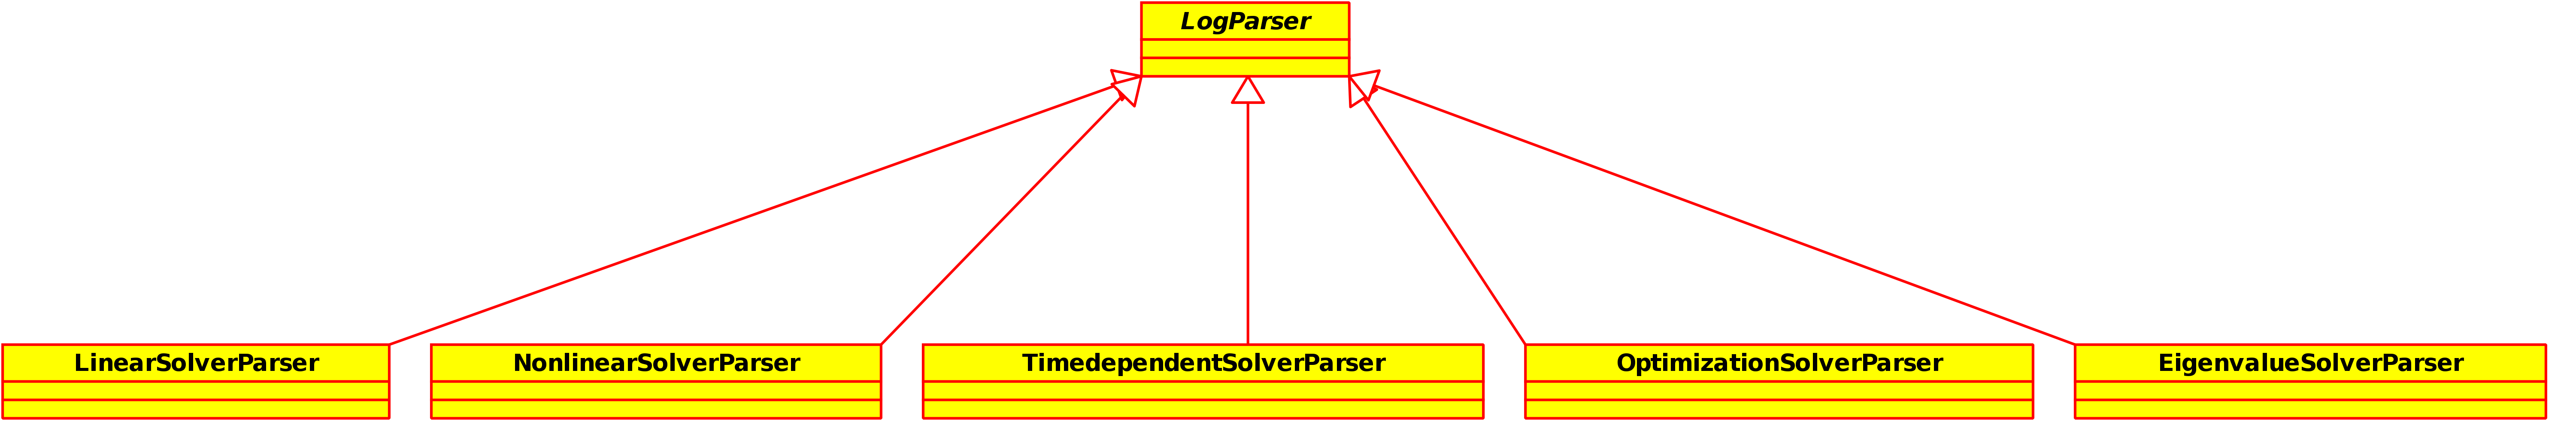
\includegraphics[keepaspectratio=true,width=\textwidth]{res/Klassendiagramm_CalculationAgent_Parser.png}
		\caption{Parser-Struktur des \calcag{}en}
		\label{calcag_parser}
	\end{figure}
	
	Der \calcag{} leitet die gelesenen Daten an den \repag{}en zur Darstellung weiter.
	
	\section{Prozessparameter-Verwaltung}\label{kap_implParver}
	Der Entwurf der Prozessparameter-Verwaltung wurde in Kapitel \ref{kap_entw_parver} beschrieben. Die Umsetzung wird in den folgenden Kapiteln erläutert. Dabei wird beleuchtet, wie der \repag{} seine Daten erhält, die Darstellung dieser wird in Kapitel \ref{kap_impl_gui} beschrieben. Die konkrete Implementierung des Datentransfers ist in Anhang \ref{kap_dataman_austausch} skizziert.
	
	\subsection{Registrierung}
	Die darzustellenden Prozessparameter werden dem \repag{}en in einem Registrierungsprozess mitgeteilt. Hierzu empfängt er eine \emph{ACLMessage}\footnote{siehe Kapitel \ref{kap_messageSystem}} mit einer \emph{Conversation-ID} mit Inhalt \emph{REGISTER\_PARAMETER}\footnote{für eine voll\-stän\-dige Erklärung des Übertragungsprotokolls siehe Anhang \ref{kap_protocol}}. Durch diesen Empfang wird ein neuer Prozessparameter registriert, welcher im Inhalt der Nachricht spezifiziert wird. Der \repag{} erwartet ein \emph{Parameter}-Objekt (siehe Anhang \ref{kap_impCl}). Hier wird, wie bereits in Kapitel \ref{kap_implDataMesh}, die FIPA-Spezifikation verletzt. Die Begründung ist analog. Das übergebene Parameter-Objekt kann bei der Registrierung bereits darzustellende Daten enthalten.
	
	\subsection{Update}\label{kap_implParverUpdate}
	Einem Prozessparameter können Daten zur Laufzeit hinzugefügt werden. Der \repag{} hat dabei die Aufgabe, die über das Netzwerk empfangenen Daten in seine Datenhaltung zu integrieren. Die GUI des Agenten ist für eine entsprechende Aktualisierung selbst verantwortlich.
	
	\subsection{Deregistrierung}
	Jedes Parameter-Objekt enthält eine für den Prozessparameter kennzeichnende ID. Wird diese in Verbindung mit der ACL-Message-Conversation-ID\footnote{siehe Kapitel \ref{kap_messageSystem}} \emph{UNREGISTER\_PARAMETER} erhalten, so wird das dazu gehörige Parameter-Objekt aus der Datenhaltung des \repag{}en entfernt.
	
	\chapter{Anwendungsbeispiel}
	In diesem Kapitel soll die vorhandene Agenten-Plattform dazu genutzt werden, um ein beispielhaftes elektrotechnisches Problem zu lösen. Dabei wird der \repag{} mit all seinen Funktionen dargestellt und dessen Funk\-tions\-fä\-hig\-keit überprüft. Das Problem ist dabei sehr einfach gehalten, um eine Konzentration auf den \repag{}en zu ermöglichen.
	
	\section{Problem}
	Gesucht ist im Folgenden das sich einstellende elektrische Feld zweier Kugelelektroden, welche im Abstand von 5\,cm voneinander entfernt eine Potentialdifferenz von 1\,V aufweisen. Beide Elektroden weisen einen Radius von 1\,cm auf. Sie werden als perfekte elektrische Leiter angenommen. Eine Kugelelektrode ist geerdet.
	
	\section{Modell}
	Modelliert wird mit \textsc{Comsol} Multiphysics\footnote{Für mehr Informationen: \citeUrls{COMSOL}} Version 4.3. Das Modell wird dabei nach den Anforderungen des beschriebenen Problems erstellt. Das entstandene Modell ist in Abbildung \ref{fig_bsp_model} zu sehen.
	\begin{figure}[ht]
		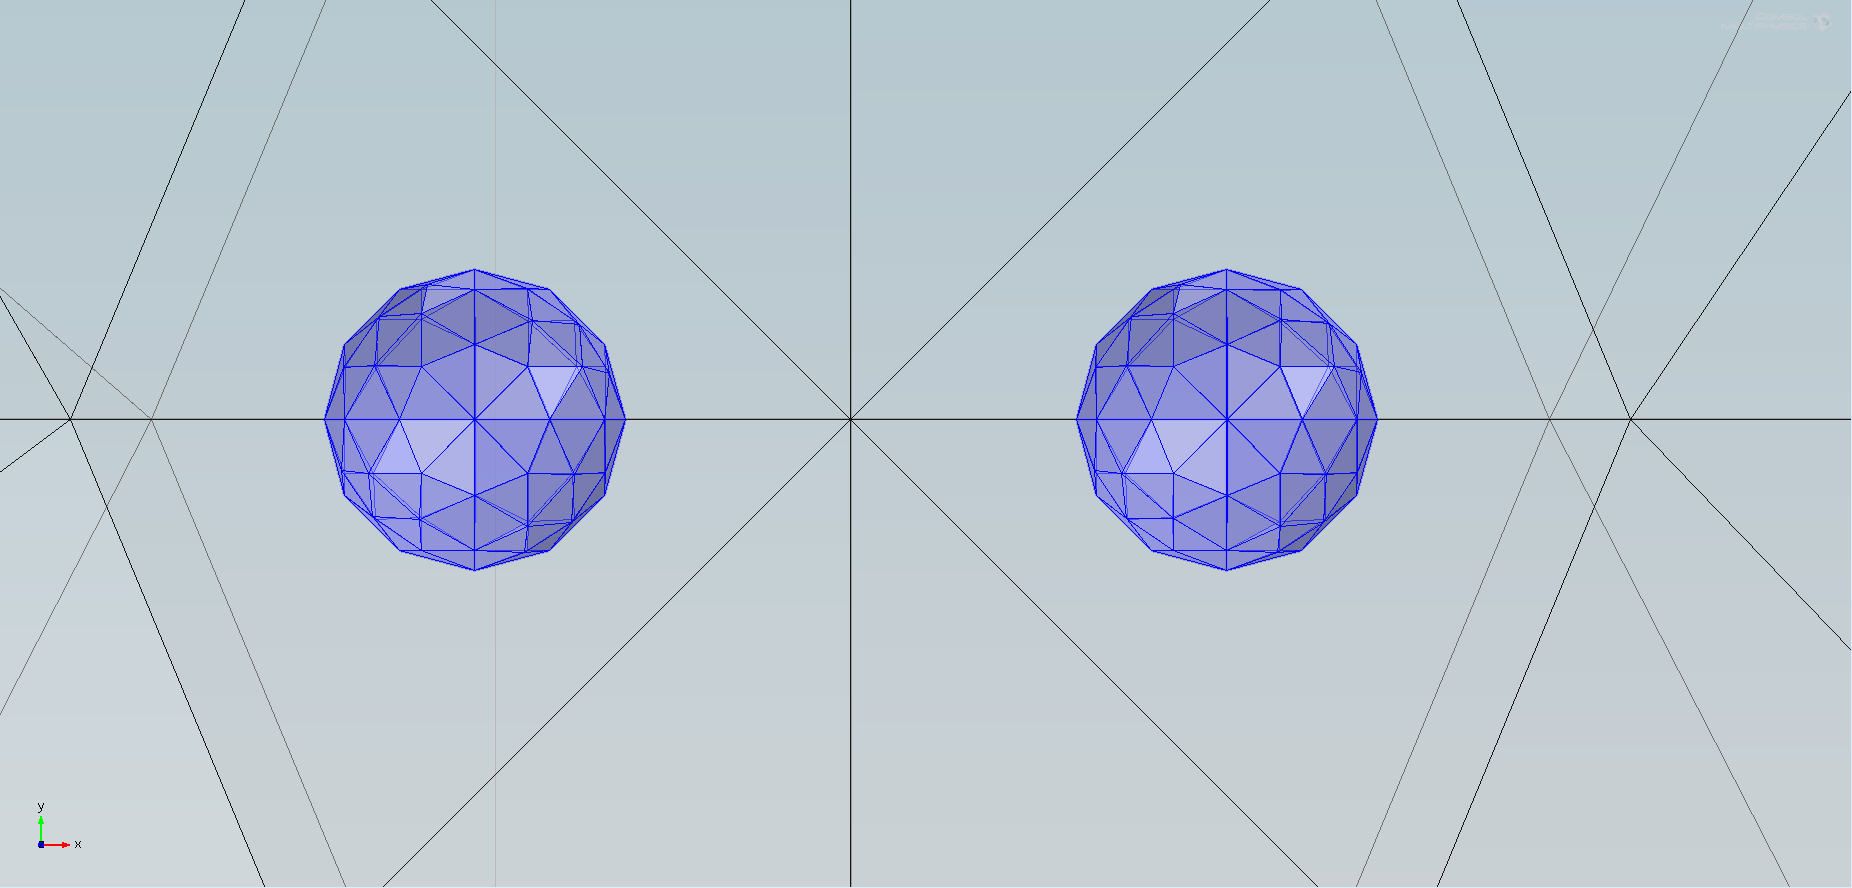
\includegraphics[keepaspectratio=true,width=\textwidth]{res/bsp_model.png}
		\caption{Modell des Anwendungsbeispiels}
		\label{fig_bsp_model}
	\end{figure}
	
	\section{Berechnung}
	Die Berechnung selbst geschieht nach Start der Agenten-Plattform. Zunächst wird das Modell geladen, anschließend wird die Berechnung durchgeführt. Beides zusammen benötigt ca. 60 Sekunden (siehe Abbildung \ref{fig_bsp_mon}). Das reine Berechnen dauert 16 Sekunden, \textsc{Comsol} berechnet das Modell in ca. 13 Sekunden. Um über die Effektivität des Systems eine Aussage treffen zu können, müsste die Berechnung genauer untersucht werden. Dies ist jedoch nicht Gegenstand dieser Arbeit.\parag{}
	\begin{figure}[ht]
		\centering
		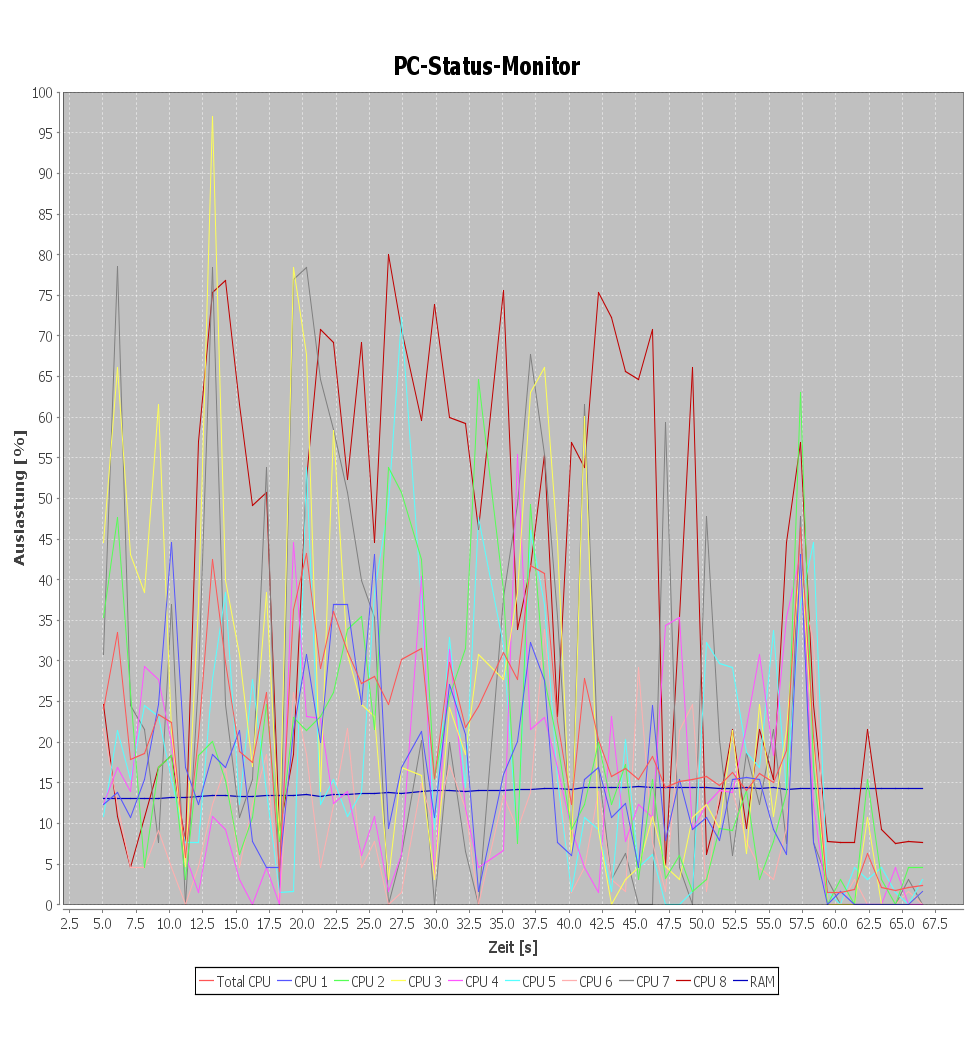
\includegraphics[keepaspectratio=true,width=0.48\textwidth]{res/bsp_statusmon.png}
		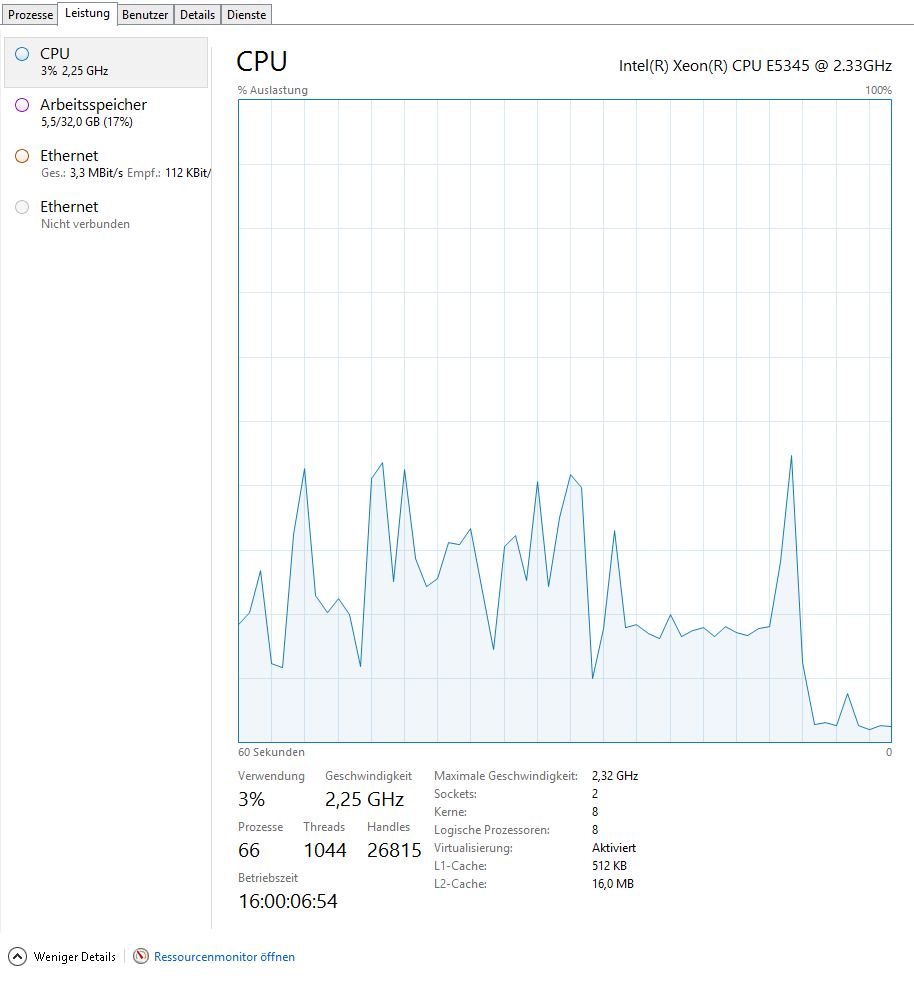
\includegraphics[keepaspectratio=true,width=0.48\textwidth]{res/bsp_taskmgr.png}
		\caption[Rechner-Auslastung bei der Berechnung des Anwendungsbeispiels]{Rechner-Auslastung bei der Berechnung des Anwendungsbeispiels -- links: PCStatusMonitor, rechts: TaskManager}
		\label{fig_bsp_mon}
	\end{figure}
	Abbildung \ref{fig_bsp_mon} zeigt die CPU- und RAM-Auslastung im Vergleich zwischen dem in dieser Arbeit implementierten \emph{PCStatusMonitor} und dem Windows-Bord\-mittel \emph{TaskManager}. Hier ist erkennbar, dass die CPU-Auslastung in etwa denselben Verlauf besitzt. Die RAM-Auslastung variiert zwischen StatusMonitor und TaskManager um ca.
	\[
		17\,\% - 14\,\% = 3\,\%,
	\]
	was einer absoluten Differenz von
	\[
		0{,}03 \cdot 32\,\text{GB} \approx 1\,\text{GB}
	\]
	entspricht. Der Rechner verfügt dabei über 32\,GB Arbeitsspeicher. Grund hierfür kann ein Fehler in \emph{SIGAR} sein. Dennoch ist eine Tendenz ablesbar, was die Information für den StatusMonitor brauchbar macht. Hier ist auch in Abbildung \ref{fig_bsp_mon} ablesbar, dass während des Ladens und Berechnens der Arbeitsspeicher um ca. 1,5\,\% zunimmt, was einen effektiven Arbeitsspeicherverbrauch von ca.
	\[
		0{,}015 \cdot 32\,\text{GB} \approx 500\,\text{MB}
	\]
	
	bedeutet. Im Rahmen der Ablesbarkeit ist dies in etwa die von \textsc{Comsol} angegebene Arbeitsspeicherbelegung.\parag{}
	\begin{figure}[ht]
		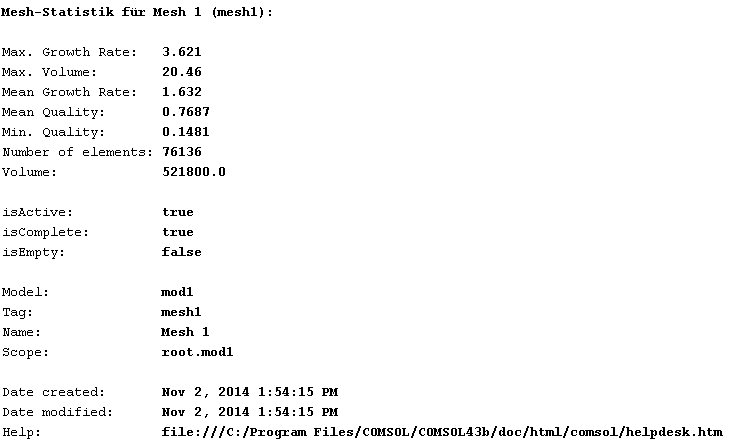
\includegraphics[keepaspectratio=true,width=\textwidth]{res/bsp_mesh.png}
		\caption{Mesh-Statistik des Anwendungsbeispiels}
		\label{fig_bsp_mesh}
	\end{figure}
	Die Statistik des Meshes aus dem Anwendungsbeispiel ist in Abbildung \ref{fig_bsp_mesh} dargestellt. Dieses ist weitgehend vollautomatisch generiert, daher sind nur wenige Informationen dargestellt. Zur Erinnerung: Felder ohne Belegung, beispielsweise das Feld \emph{Autor}, werden vom \repag{}en ignoriert.
	
	\begin{figure}[ht]
		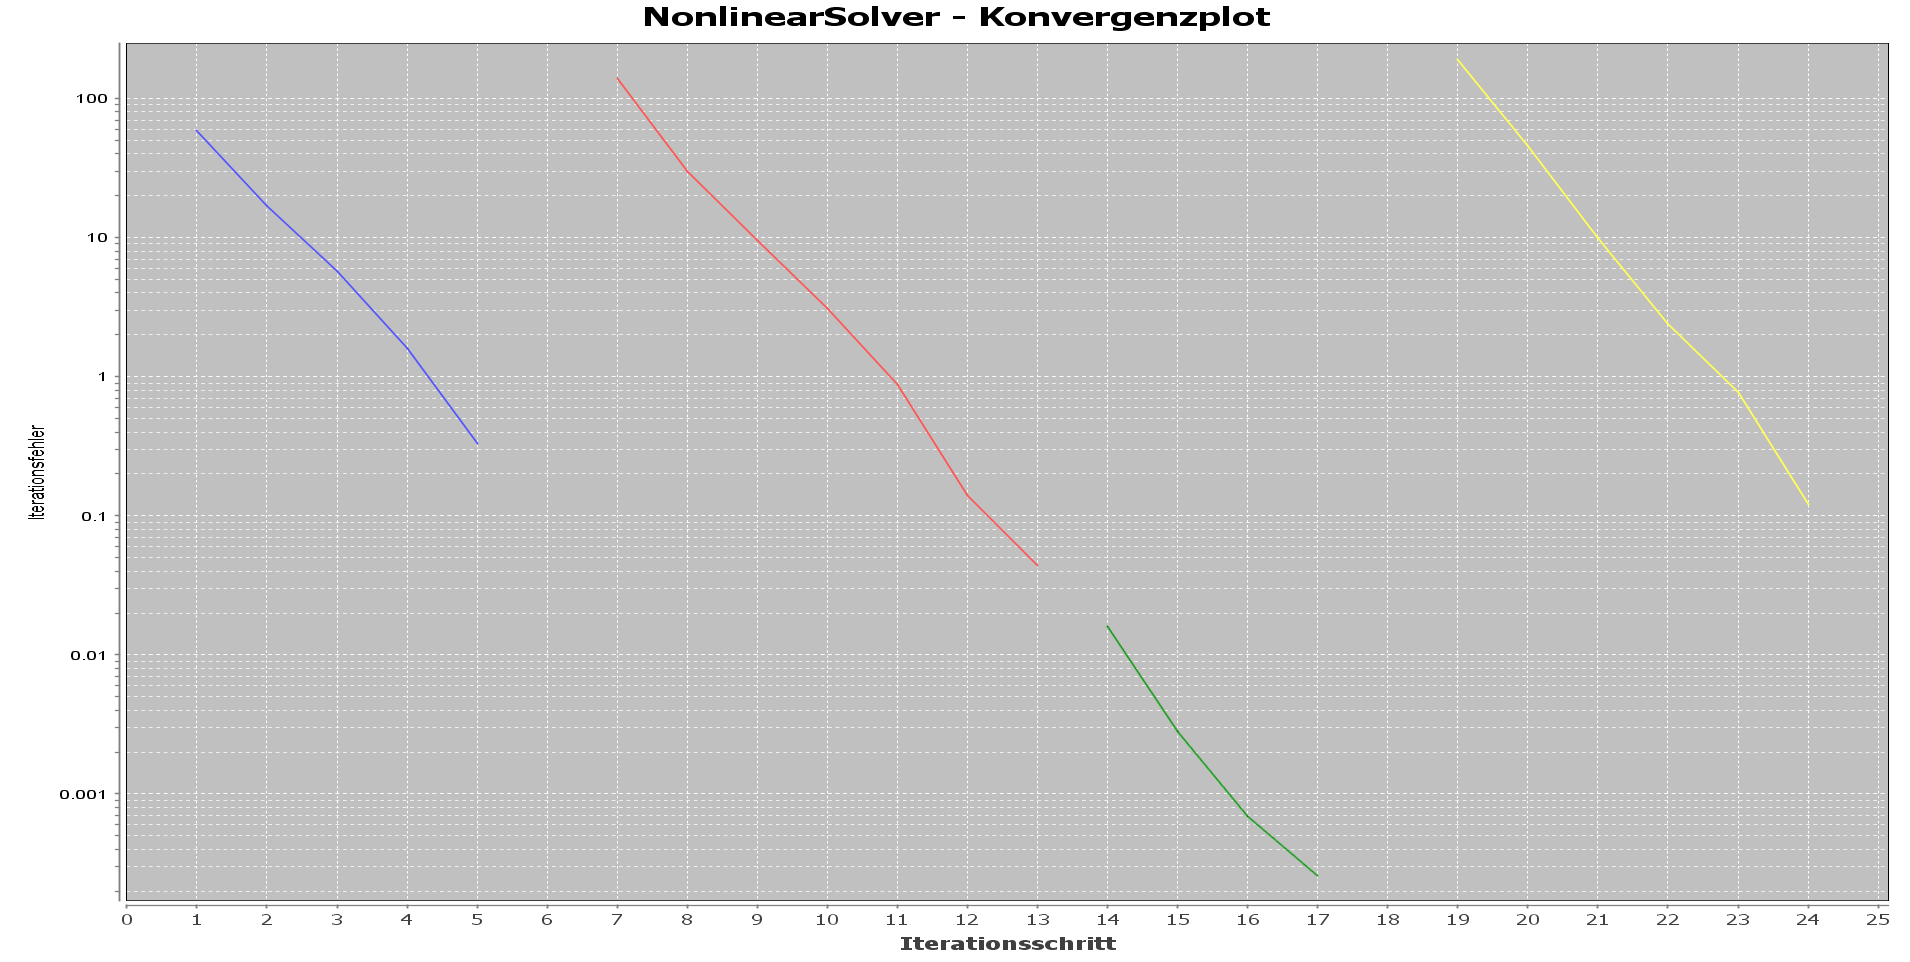
\includegraphics[keepaspectratio=true,width=\textwidth]{res/bsp_konvplot.png}
		\caption{Konvergenzdiagramm des Anwendungsbeispiels}
		\label{fig_bsp_konvplot}
	\end{figure}
	\begin{figure}[ht]
		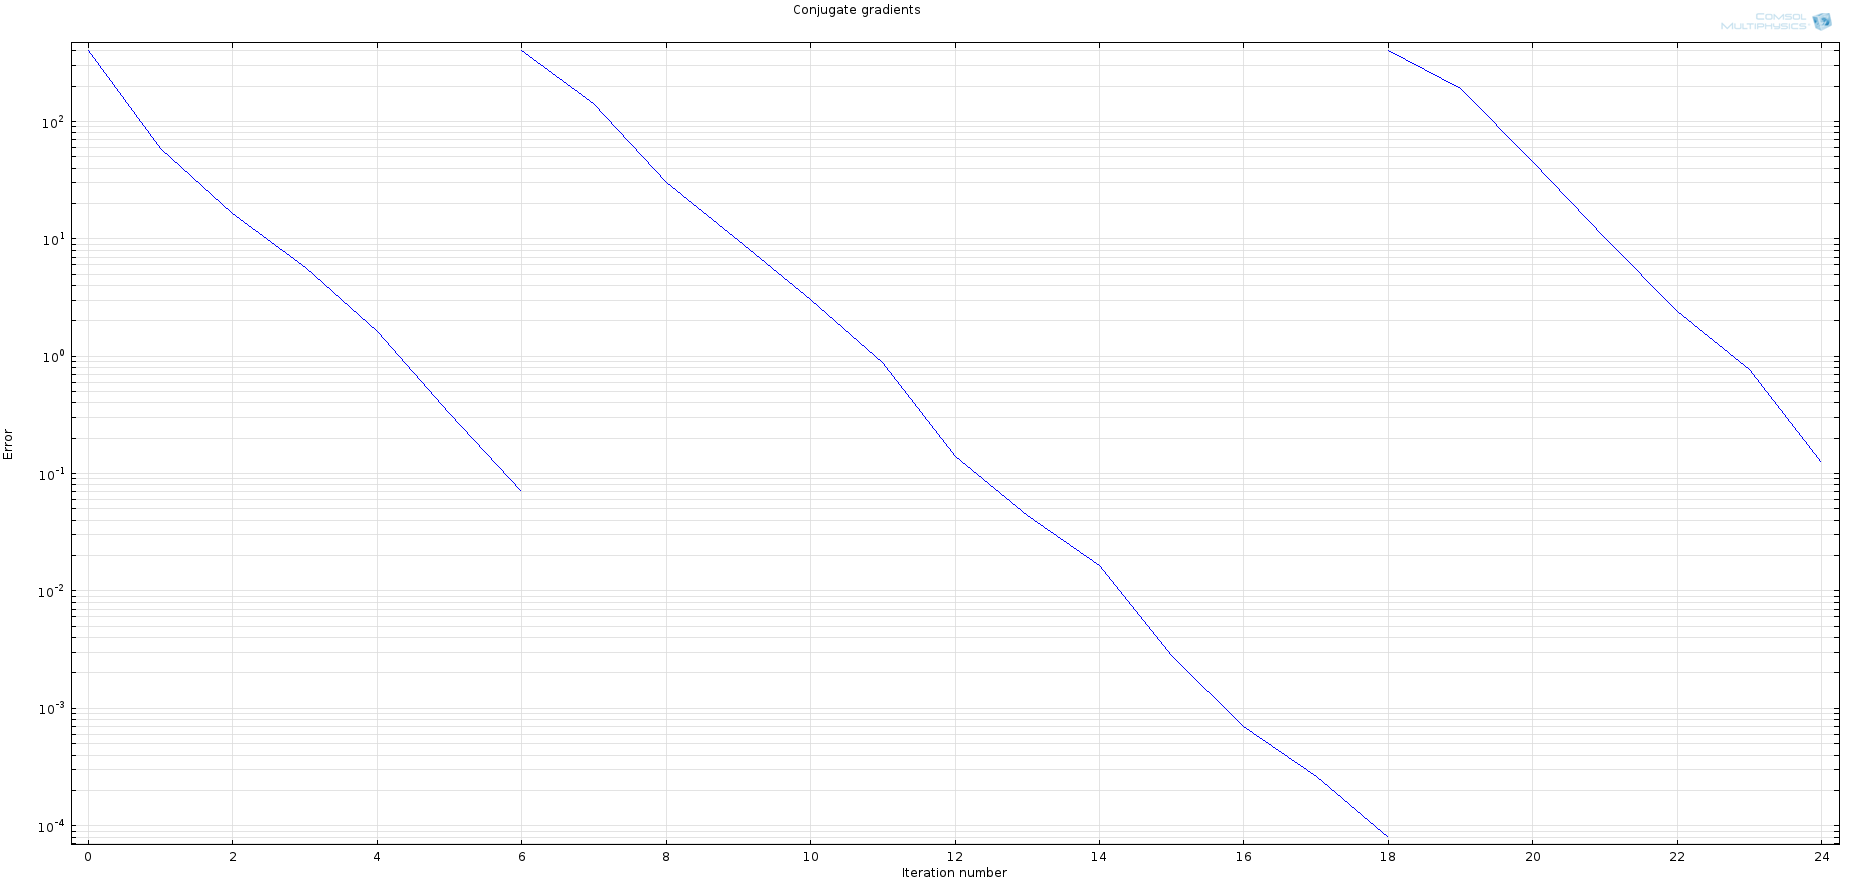
\includegraphics[keepaspectratio=true,width=\textwidth]{res/bsp_konvplot_comsol.png}
		\caption[Konvergenzdiagramm des Anwendungsbeispiels (\textsc{Comsol})]{Konvergenzdiagramm des Anwendungsbeispiels bei der Berechnung mit \textsc{Comsol}}
		\label{fig_bsp_konvplot_comsol}
	\end{figure}
	Das zugehörige Konvergenzdiagramm ist in Abbildung \ref{fig_bsp_konvplot} zu finden. Er wurde vom \repag{}en gezeichnet. Abbildung \ref{fig_bsp_konvplot_comsol} zeigt das Konvergenzdiagramm von \textsc{Comsol}, welcher dieses bei der Berechnung desselben Modells erzeugt. Man sieht eine sehr starke Ähnlichkeit, somit kann das vom Agenten gezeichnete Diagramm als äquivalent betrachtet werden.
	
	\section{Ergebnis}
	Die Agenten-Plattform, mit der an dieser Stelle gearbeitet wurde, ist eine vereinfachte Version, daher kann das Simulationsergebnis nicht dargestellt werden. Der \repag{} ist davon jedoch nicht betroffen, er findet die gleichen Schnittstellen vor wie in der eigentlichen Version der ITE-Agentenplattform.

	\chapter{Zusammenfassung und Ausblick}\label{kap_ausblick}
	Das Hauptziel dieser Arbeit besteht darin, ein Programm zu schaffen, welches in einfacher Weise Prozessparameter aus einer Agentenplattform zur Simulation numerischer Probleme extrahieren und darstellen kann. Dabei soll die Benutzeroberfläche intuitiv, einfach gestaltet und leicht zu bedienen sein. Das Design der Oberfläche soll ansprechend und in sich geschlossen wirken.\parag{}
	Der in dieser Arbeit entwickelte Agent besitzt die Fähigkeit, Prozessparameter zu empfangen, zu speichern und graphisch darzustellen. Obzwar die Daten statistisch nicht ausgewertet werden, wird dies durch die Diagramme wesentlich erleichtert. Die Benutzeroberfläche verzichtet auf Menüs, hierdurch lässt sich die Oberfläche einfach und ohne Vorkenntnisse bedienen. Die meisten Registerkarten sind dabei mit Icons versehen, welche eine Bedienung ohne das Lesen von Text ermöglichen. Damit wird eine intuitive Bedienbarkeit ermöglicht. Die grafische Benutzeroberfläche visualisiert das Agenten-System durch die Fensteraufteilung in geeigneter Weise. Dies ermöglicht auch den direkten Vergleich von Prozessparametern verschiedener Agenten.\parag{}
	Der hier entwickelte Agent erfüllt damit die an ihn gestellten Anforderungen. Allerdings gehen die theoretischen Möglichkeiten des Agenten über die in dieser Arbeit entwickelten weit hinaus. Diese Erweiterungen werden im Folgenden erläutert.

	\section{Auswerten der Daten}
	Der \repag{} könnte die Daten, die er von den anderen Agenten bekommt, auswerten und entsprechend reagieren. Hierdurch ließe sich beispielsweise eine höhere Stabilität oder eine höhere Effizienz des Agenten-Systems erreichen. Durch den PC-Status-Monitor kann der jeweilige Rechner überwacht werden. Dies lässt in Grenzen Rückschlüsse auf die \glqq{}Gesundheit\grqq{}, also die Funktionsfähigkeit, des Systems zu. Wird ein Defekt erkannt, so kann versucht werden, diesen zu beheben. Sollten die Grenzen des Agenten erreicht sein, so können Mitteilungen in Form von SMS, E-Mail oder Ähnlichem erfolgen. Hierdurch kann wertvolle Zeit gespart werden, die zwischen dem Auftreten des Fehlers und dessen Entdeckung vergeht. Mögliche Beispiele für Anwendungen sind:
	\begin{itemize}
		\item Neustart des Agenten, wenn diese sich nicht rückmelden
		\item Portierung des Agenten auf einen anderen Rechner, um vorhandene Rech\-ner-Ka\-pa\-zi\-tät\-en möglichst effizient auszunutzen
		\item Warnmeldung oder eine geeignete Ereignisbehandlung, falls einzelne Rechner nicht genutzt werden
		\item Warnmeldung, E-Mail-Mitteilung oder Ähnliches, wenn der Rechenvorgang unerwartet beendet wurde
	\end{itemize}

	\section{Weitere Funktionen}
	Der Agent kann um zusätzliche Funktionalität erweitert werden. Einige Mög\-lich\-keit\-en werden im Folgenden kurz vorgestellt.
	
	\subsection{Ausgliederung der Tabs}
	Der Vergleich von Prozessparametern verschiedener Agenten ist zurzeit problemlos mög\-lich. Doch ein Vergleich verschiedener Prozessparameter desselben Agenten gestaltet sich schwierig, da stets zwischen verschiedenen Tabs gewechselt werden muss. Es ist daher empfehlenswert, die GUI so anzupassen, dass dieses Problem gelöst werden kann. Ein möglicher Ansatz besteht dabei, die Tabs auf Mausklick ebenfalls als \emph{Dockable} auszugliedern. Hierdurch wird die Flexibilität vergrößert, allerdings ist dann die Zuordnung eines Prozessparameters zu einem Agenten nicht zweifelsfrei möglich. Abhilfe kann hier der Einsatz von Farben schaffen.
	
	\subsection{Filterfunktion der Konsole}\label{kap_KonsoleFilter}
	Die Konsole ist momentan in der Lage, Text -- je nach Wichtigkeit verschieden formatiert -- darzustellen. Für eine bessere Übersichtlichkeit, ist ein Filter, mit dem unwichtigere Nachrichten ausgeblendet werden können, vorteilhaft. Dieser würde Betrieb und Fehlersuche gleichermaßen erleichtern.
	
	\subsection{Suchfunktion der Konsole}
	Eine weitere Erweiterung für die Konsole stellt eine Suchfunktion dar. Diese Funktion wird voraussichtlich weniger gebraucht, ist jedoch heute nahezu überall zu finden (Browser, Dokumentenbetrachter, Dateimanager, \ldots{}). Sie kann im Einzelfall enorm Zeit sparen und ist mit nicht allzu hohem Aufwand implementierbar, daher wird sie dennoch als sinnvoll eingestuft. In Kombination mit der vorgestellten Filterfunktion (Kapitel \ref{kap_KonsoleFilter}) kann die Suchfunktion treffende Ergebnisse liefern.
	
	\subsection{Export der Konsole}
	Eine weitere nützliche Funktion ist der Export des Konsoleninhaltes in eine Datei. Hierdurch könnten verschiedene Anwendungsfälle gespeichert und verglichen werden. Auch die Fehlersuche wäre damit wesentlich leichter, vor allem im produktiven Einsatz des Systems.\\
	Ein Export ist bereits durch die Tastenkombination [Strg]+[C] in die Zwischenablage möglich, jedoch geht hierbei die Formatierung des Textes verloren. Ein sehr effektives System wäre der Export der Konsole in Kombination mit der Filterfunktion (Kapitel \ref{kap_KonsoleFilter}), denn so kann der Export des Konsoleninhaltes auf den entscheidenden Inhalt beschränkt werden.
	
	\subsection{Export der Diagramme}
	Die Speicherung der Diagramme ist bislang nur über einen \emph{Screenshot}\footnote{Bildschirmaufnahme in Form eines Bildes} möglich. Diese Fähigkeit zur Speicherung von Diagrammen wird häufig benötigt, beispielsweise für Präsentationen. Der Screenshot muss nachbearbeitet werden, da er nicht nur das Diagramm enthält. Daher wäre die gezielte Speicherung einzelner Diagramme per Knopfdruck als Bild oder PDF evtl. mit den Datensätzen eine äußerst nützliche Funktion.

	% creating appendix
	\appendix
	\chapter{Datenmanagement}
	Dieses Kapitel erläutert einige bedeutende Aspekte der Implementierung des \repag{}en. Diese sind sehr speziell und werden daher nur benötigt, wenn der Quelltext verstanden werden will.
	
	\section{Text-Level}\label{kap_textlevels}
	Da die Konsole eine formatierte Ausgabe erlaubt, wurden sogenannte \emph{Text-Level} eingeführt. Diese lauten (von wichtig zu unwichtig):
	
	\begin{enumerate}
		\item \emph{Fatal}: Das Problem, welches diese Nachricht verursacht, bringt das Programm zum Absturz.
		\item \emph{Error}: Dieses Problem kann nicht ignoriert werden. Das Programm läuft dennoch fort.
		\item \emph{Warning}: Das aufgetretene Problem kann ignoriert werden.
		\item \emph{Information Important}: Der Text beinhaltet eine wichtige Information für den Benutzer.
		\item \emph{Information Casual}: Der Text beinhaltet eine beiläufige Information für den Benutzer, welche dieser nicht unbedingt benötigt.
		\item \emph{Debug}: Der Text dient ausschließlich als Debug-Information. Der Benutzer sollte diese Information nicht sehen.
		\item \emph{Unknown}: Falls kein Text-Level definiert ist oder sonstige Fehler bei dessen Dekodierung auftreten.
	\end{enumerate}
	
	\section{Wichtige Klassen}\label{kap_impCl}
	\paragraph{reportagent.stats.Parameter}
	Repräsentiert einen Datensatz mit sämtlichen Informationen, die zur Darstellung eines Prozessparameters erforderlich sind, \zB{} den Diagramm-Typ. Das zur Klasse zugehörige Attribut \emph{parameterID} definiert klar den Typ des Prozessparameters, \zB{} Fortschritt.\parag{}
	\emph{Hinweis:} Dieses Attribut darf keinesfalls mit dem Attribut \emph{type} verwechselt werden, welches den \emph{Diagramm-Typ} spezifiziert, also \zB{} ein XY-Chart.

	\paragraph{reportagent.stats.ParameterMap}
	Abstrakte Klasse, die Informationen über einzelne Parametertypen enthält, beispielsweise das X-Achsen-Label des Parameters \emph{PCStatus}.

	\paragraph{reportagent.ProtocolRA}
	Interface, welches Konstanten beinhaltet. Diese definieren das Übertragungsprotokoll (siehe Kapitel \ref{kap_protocol}).

	\section{Das Übertragungsprotokoll}\label{kap_protocol}
	Übertragen werden müssen folgende Kommandos:

	\paragraph{REGISTER\_PARAMETER}
	Befehl zur Registrierung eines neuen Prozessparameters beim \repag{}en. Es wird erwartet, dass in der ACLMessage als \emph{ContentObject} ein Objekt des Typs \emph{Parameter} vorliegt.

	\paragraph{UNREGISTER\_PARAMETER}
	Befehl zum Löschen eines Prozessparameters. Wieder wird als \emph{ContentObject} ein Objekt vom Typ Parameter erwartet.

	\paragraph{UPDATE\_PARAMETER}\label{kap_UpdateMsg}
	Befehl zum Update eines Prozessparameters. Die Syntax lautet:

	\begin{lstlisting}[caption={Syntax UPDATE\_PARAMETER},label={lst_syntax_datentag}]
		<parameterID>;<Daten>
	\end{lstlisting}

	wobei der Tag \textit{Daten} frei spezifiziert werden darf. Der Code zur Interpretation dieser Zeile findet sich dabei in der Klasse \emph{reportagent.""behaviours.""Update"-Msg"-Handler}.

	\section{Austausch der Daten}\label{kap_dataman_austausch}
	Dieser Teil beschreibt die Implementierung des Datentransfers zwischen den Agenten. Diese ist sehr spezifisch und bezieht sich direkt auf die in Kapitel \ref{kap_existingPlatform} vorgestellte Beispielplattform, in die der \repag{} eingebettet ist.
	
	\subsection{Sendeseite}
	Für die Verwaltung der Daten ist der \numag{} mit der Klasse \emph{numericagent.InformationManager} ausgestattet. Die Klasse \emph{InformationManager} besitzt die Methode \emph{addParameter(\ldots)}, die den \repag{}en über einen neuen Prozessparameter informiert. Ferner besitzt der \emph{InformationManager} die Methode \emph{update(\ldots)}, die zuerst \emph{addParameter(\ldots)} aufruft, wenn nicht bereits geschehen. Anschließend wird der \repag{} über die neuen Daten informiert.\parag{}
	Da der \calcag{} von \numag{} erbt, steht ihm diese Klasse ebenfalls zur Verfügung. Zu beachten ist, dass im Design davon ausgegangen wurde, dass es von dieser Klasse nur ein Objekt gibt, dies jedoch nicht sichergestellt wurde. Hintergrund ist, dass es mehrere Instanzen des \repag{}en geben kann. Weiter läuft man bei der Programmierung keine Gefahr, mehrere Instanzen der Klasse \emph{InformationManager} zu erzeugen.

	\subsection{Empfangsseite}
	Die Parameter, die neu registriert werden, werden in dem \repag{}en hinterlegt. In der GUI wird ein neuer Tab mit dem entsprechenden Parameter angelegt. Zu beachten ist, dass ein \repag{} mehrere \numag{}en kennen kann und jeder \numag{} mehrere Parameter besitzen kann. Dies ist in der Datenstruktur zur Speicherung der Parameter berücksichtigt, es ergibt sich das Klassendiagramm aus Abbildung \ref{repag_params}.
	\begin{figure}[ht]
		\centering
		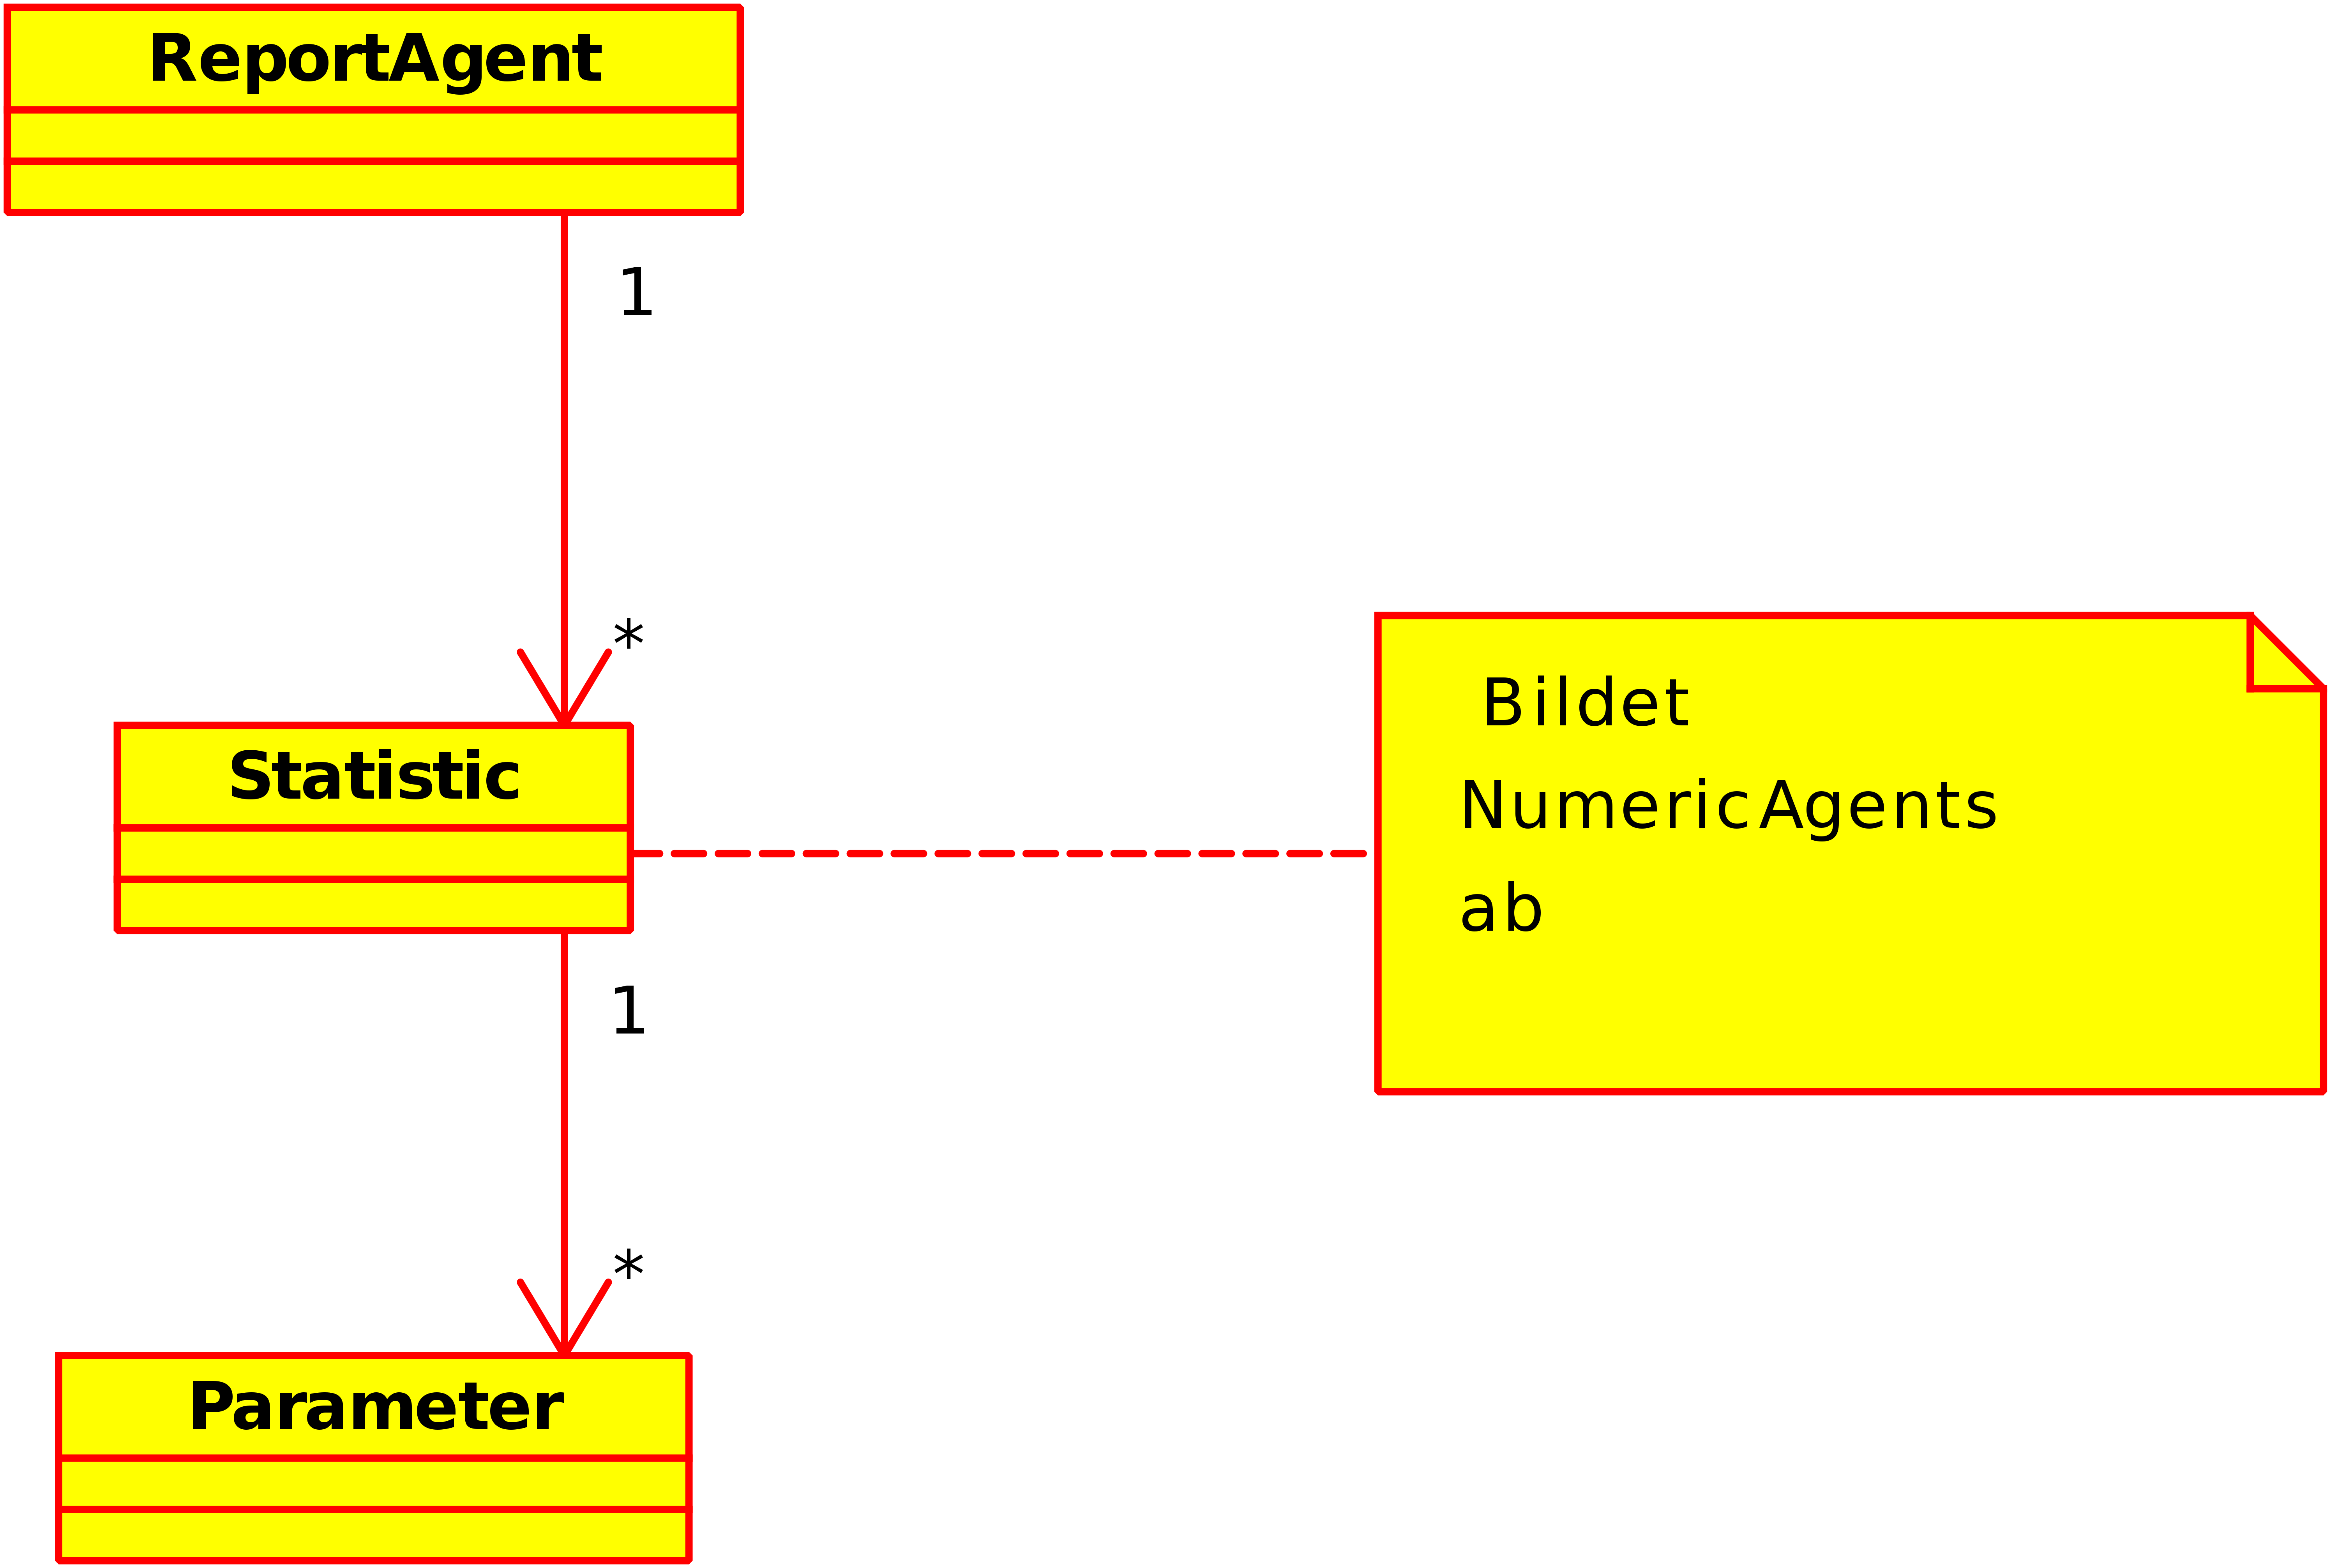
\includegraphics[keepaspectratio=true, width=\textwidth]{res/Klassendiagramm_ReportAgent_Parameterverwaltung.png}
		\caption{Parameterverwaltung des \repag{}en}
		\label{repag_params}
	\end{figure}\parag{}
	Wird nun ein neues Datum empfangen, so wird ein neuer Parameter registriert oder ein bestehender aktualisiert. Die GUI aktualisiert sich in diesem Fall automatisch.
	
	\chapter{Hinzufügen von Prozessparametern}\label{kap_AddParameter}
	Für das nachträgliche Hinzufügen von Parametern in das System müssen lediglich wenige Stellen im Programmtext bearbeitet werden. Diese werden im Folgenden kurz vorgestellt. Da dieses Kapitel als Programmieranleitung gedacht ist, wird für dessen Verständnis Zugang und Verständnis des Quelltextes vorausgesetzt.
	
	\section{Weiterleitung an den \repag{}en}
	Es wird davon ausgegangen, dass die Daten bereits abrufbar sind. Diese müssen an den \repag{}en übergeben werden. Dies geschieht durch die Klasse \emph{numericagent.InformationManager} mit der Methode \emph{addParameter(\ldots)}. Diese ist überladen (siehe \lstlistingname{} \ref{lst_InfoMgr_addParam}).
	\begin{lstlisting}[caption={Auszug aus numericagent.InformationManager},label={lst_InfoMgr_addParam}]	
public void addParameter(Parameter p) {
	...
}

public void addParameter(int paramID) {
	addParameter(new Parameter(paramID));
}
	\end{lstlisting}
	In der einen Version erwartet sie einen Parameter vom Typ \emph{reportagent.stats.Pa\-ra\-me\-ter}, in der anderen einen Parameter vom primitiven Typ \emph{Integer}. Dabei erzeugt die Methode mit dem primitiven Parameter ein neues \emph{Parameter}-Objekt und übergibt dieses an die andere Methode. Obwohl ein Fehlerfall nicht über\-prüf\-bar ist, kann davon ausgegangen werden, dass nach Aufruf dieser Methode das \emph{Parameter}-Objekt korrekt an \repag{} übergeben wurde. Aufgetretene Fehler wird die \emph{update(\ldots)}-Methode beheben.
	
	\section{Parameter}
	Um die \emph{addParameter(\ldots)}-Methode des \emph{InformationManagers} aufrufen zu kön\-nen, wird mindestens eine \emph{parameterID} benötigt (siehe \lstlistingname{} \ref{lst_InfoMgr_addParam}). Diese sollte in der Klasse \emph{Parameter} als Konstanten definiert werden. Dabei ist der Wert in Grenzen frei wählbar -- er sollte zwischen 1 und 2000 liegen. Ein Beispiel ist die Konstante \emph{Parameter.PROGRESS}, die einen Wert von 100 aufweist.\parag{}
	Die genauere Definition des Parameters (Diagramm-Typ, Achsen-Be\-schrif\-tung\-en,\ldots) werden in der Klasse \emph{reportagent.stats.ParameterMap} vorgenommen. Dabei sollten mindestens die Methoden \emph{getParameterType(\ldots)}, \emph{getParameterTitle(\ldots)} und \emph{getParameterDataset(\ldots)} erweitert werden, andernfalls wird eine Warnung ausgegeben. Die Methoden sind alle nach ähnlichem Muster Aufgebaut. Ein Beispiel ist in \lstlistingname{} \ref{lst_ParameterMap_getParameterTitle} zu finden.
	
	\begin{lstlisting}[caption={reportagent.stats.ParameterMap.getParameterTitle()},label={lst_ParameterMap_getParameterTitle}]
public static String getParameterTitle(int parameterID) {
	try {
		switch (parameterID) {
		case Parameter.PROGRESS:
			return "Fortschritt";
			
		case Parameter.MEMORY:
			return "Speicherauslastung";
			
		case Parameter.PCSTATUS:
			return "PC-Status-Monitor";
			
		default:
			handleUnknownParameterError();
			return null;
		}
	} catch (Exception e) {
		return null;
	}
}
	\end{lstlisting}
	
	Hier ist zu erkennen, dass die Methoden als \emph{static} deklariert sind. Die Differenzierung der Parameter erfolgt in einer die Methode bestimmenden \emph{switch}-Verzweigung. Hier muss durch ein weiteres \emph{case}-Statement lediglich der neue Prozessparameter definiert werden. Hierbei ist die \emph{ID} des Prozessparameters, definiert in \emph{reportagent.stats.Parameter}, anzugeben.
	
	\section{Update-Messages}
	Sofern der Prozessparameter aktualisiert werden muss, muss auch die Update-Message \emph{UPDATE\_PARAMETER} definiert werden (siehe dazu Kapitel \ref{kap_UpdateMsg}). Dies geschieht sendeseitig durch einen entsprechenden Aufruf der Methode \emph{update(\ldots)} des \emph{InformationManagers}. Der übergebene Parameter \emph{updateMsg} vom Typ String muss dabei die korrekte Definition des \emph{Daten}-Tags wahren (siehe \lstlistingname{} \ref{lst_syntax_datentag}). Empfangsseitig muss die Methode \emph{action()} der Klasse \emph{reportagent.""behaviours.""Update\-Msg\-Handler} erweitert werden (siehe \lstlistingname{} \ref{lst_UpdateMsgHandler_action}). In der Methode wird zuerst geprüft, ob die Nachricht korrekt ist. Die Interpretation des \emph{Daten}-Tags findet in der großen \emph{switch}-Anweisung am unteren Ende der Methode statt.
	
	\begin{lstlisting}[caption={reportagent.behaviours.UpdateMsgHandler.action()},label={lst_UpdateMsgHandler_action}]
try {
	// Validierung und Vorverarbeitung der Nachricht
	
	switch(p.getParameterID()) {
		// Verarbeitung des Daten-Tags
		// Erweiterung hier!
	}
} catch (Exception e) {
	e.printStackTrace();
}
	\end{lstlisting}


	% -----------------------------------  list of figures   ------------------------------------------
	\clearpage
	\listoffigures{}
	\addcontentsline{toc}{chapter}{\listfigurename} % entry to toc
	
	
	% ---------------------------------  list of source codes   ---------------------------------------
	\lstlistoflistings{}
	\addcontentsline{toc}{chapter}{\lstlistlistingname} % entry to toc
	
	% -----------------------------------   bibliographies   ------------------------------------------
	\begin{flushleft}
	\bibliographyRefs{Refs}
	\addcontentsline{toc}{chapter}{\refver} % entry to toc
	
	\bibliographyUrls{Urls}
	\addcontentsline{toc}{chapter}{\webver} % entry to toc
	\end{flushleft}
\end{document}
